\documentclass[../psets.tex]{subfiles}

\pagestyle{main}
\renewcommand{\leftmark}{Homework 1}

\begin{document}




\begin{enumerate}
    \item \marginnote{4/7:}For each complex, provide the (i) oxidation state, (ii) $d^n$ configuration, and (iii) NVE (number of valence electrons, or electron count) at the metal. Provide this information for both metals and provide the number of \ce{M-M} bonds in the bimetallic cases.
    \begin{enumerate}[label={\arabic*)}]
        \item ${\color{white}hi}$
        \begin{center}
            % \chemfig{Rh(-Cl)(-[2]PPh_3)(-[4]Ph_3P)(-[6]PPh_3)}
            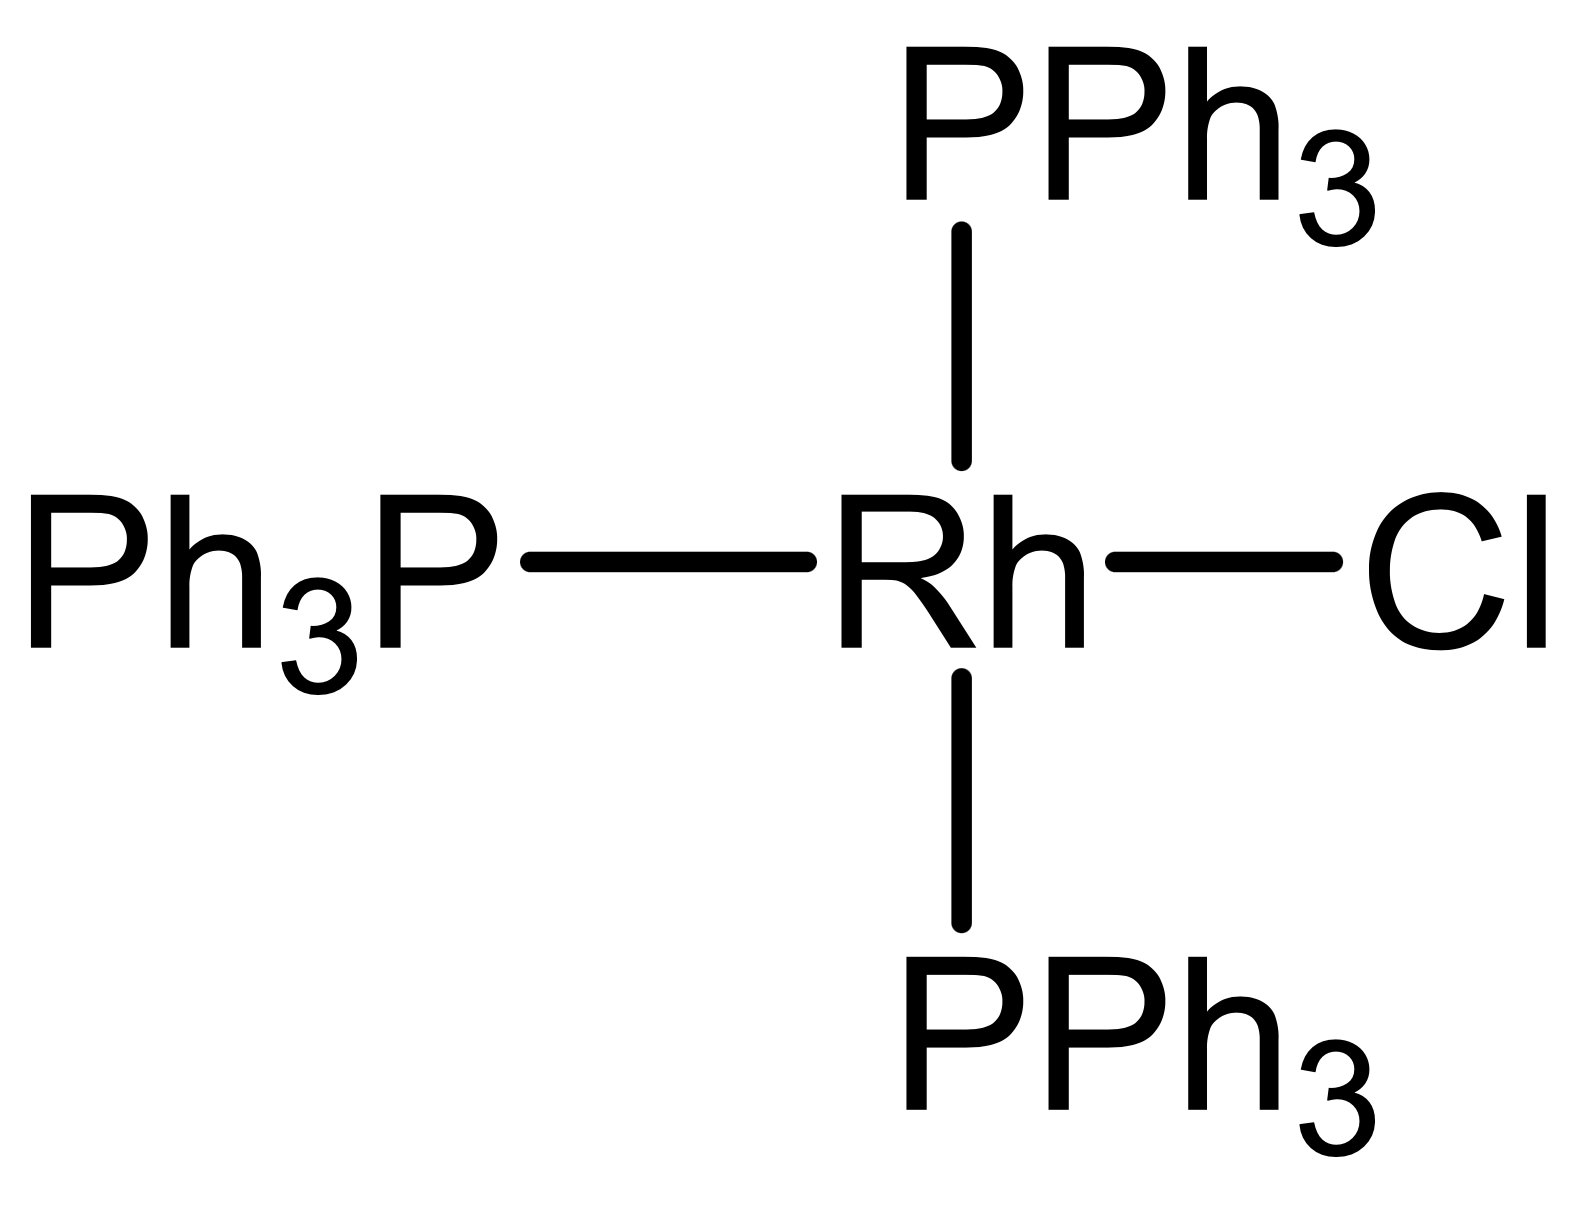
\includegraphics[width=0.2\linewidth]{../ExtFiles/pset1-1-01.png}
        \end{center}
        \begin{proof}[Answer]\leavevmode
            \begin{enumerate}[label={(\roman*)}]
                \item \ce{Rh^+} (each phosphine is L-type; the chlorine is X-type).
                \item \ce{Rh^+} is $d^8$.
                \item Each phosphine is a 2-electron donor, and the chlorine is a 1-electron donor. Thus, the ligands donate $3\cdot 2+1\cdot 1=7$ electrons in total. This combined with the above results yields $7+9=16$ as the electron count.
            \end{enumerate}
        \end{proof}
        \item ${\color{white}hi}$
        \begin{center}
            % \chemfig{Co(-\phantom{i}-[:-80,0.37,,,white]=[2]-[1])(-[2]H)(>:[:160]OC)(<[:-150]OC)(-[6]CO)}
            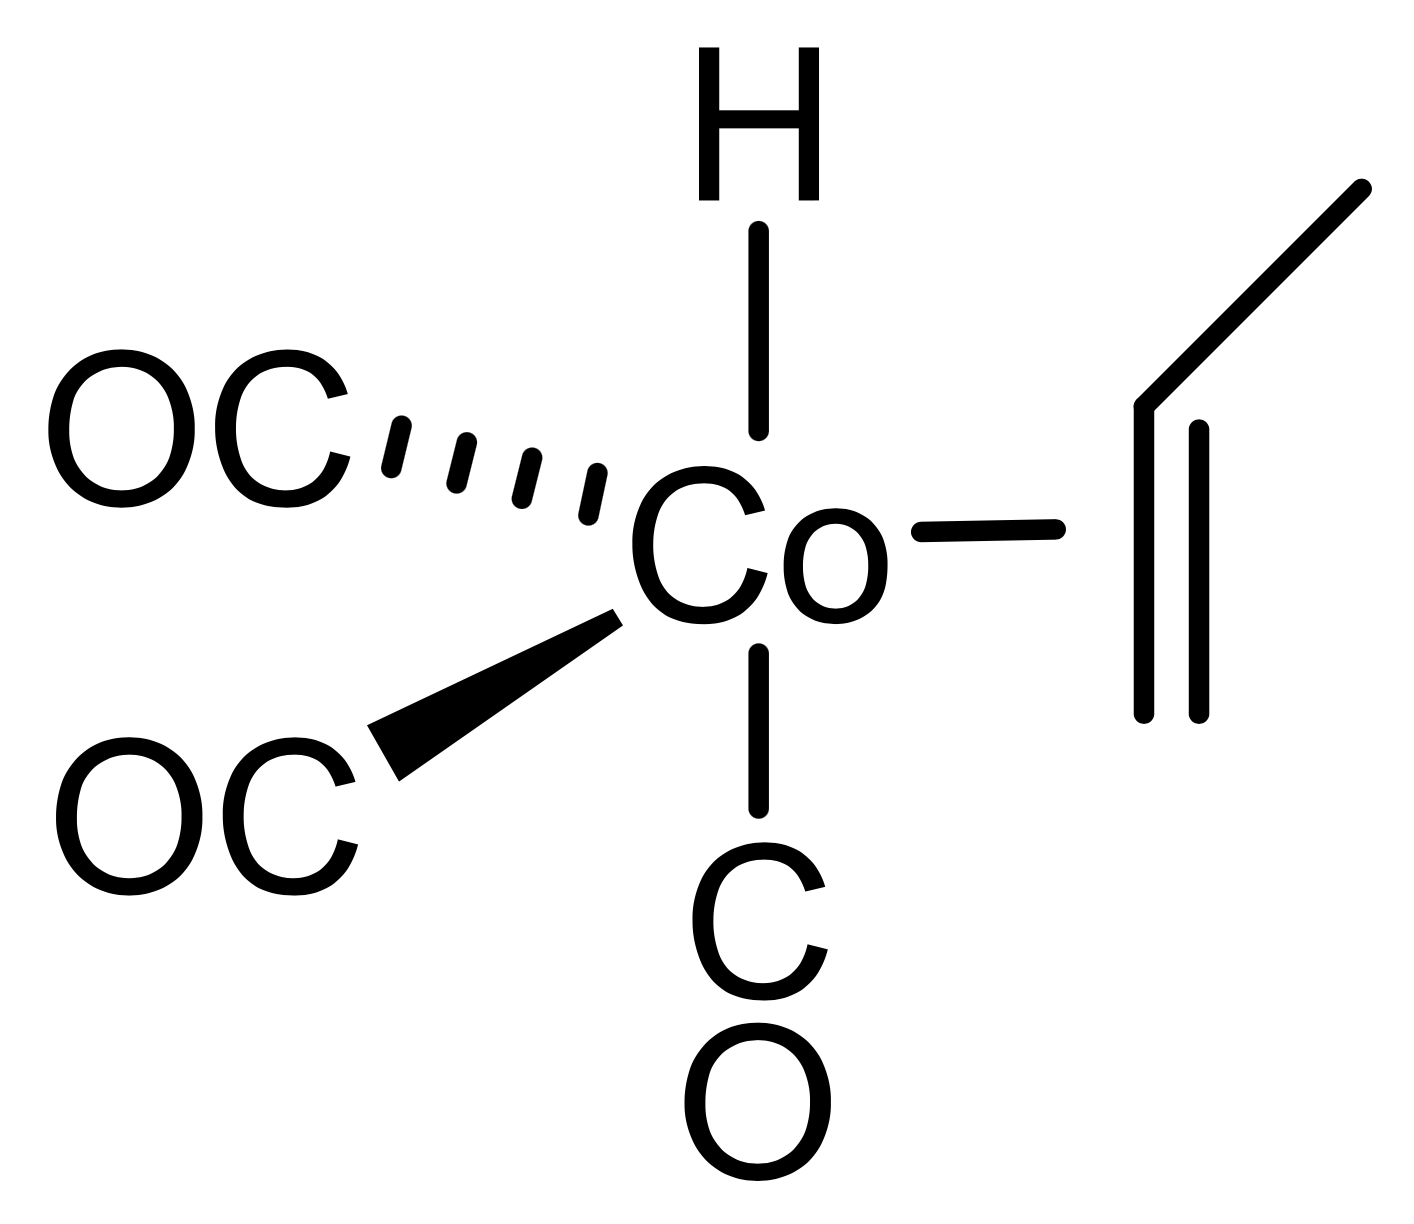
\includegraphics[width=0.2\linewidth]{../ExtFiles/pset1-1-02.png}
        \end{center}
        \begin{proof}[Answer]\leavevmode
            \begin{enumerate}[label={(\roman*)}]
                \item \ce{Co^+} (each carbonyl is L-type; the hydride is X-type; the propene is L-type).
                \item \ce{Co^+} is $d^8$.
                \item Each carbonyl is a 2-electron donor, the hydrogen is a 1-electron donor, and propene is a 2-electron donor. Thus, the ligands donate $3\cdot 2+1\cdot 1+1\cdot 2=9$ electrons in total. This combined with the above result yields $9+9=18$ as the electron count.
            \end{enumerate}
        \end{proof}
        \item ${\color{white}hi}$
        \begin{center}
            % \chemleft{[}
            %     \chemfig{Fe(-CO)(-[2]CO)(-[6]CO)(>:[:160]OC)(<[:-150]OC)}
            % \chemright{]^{2-}}
            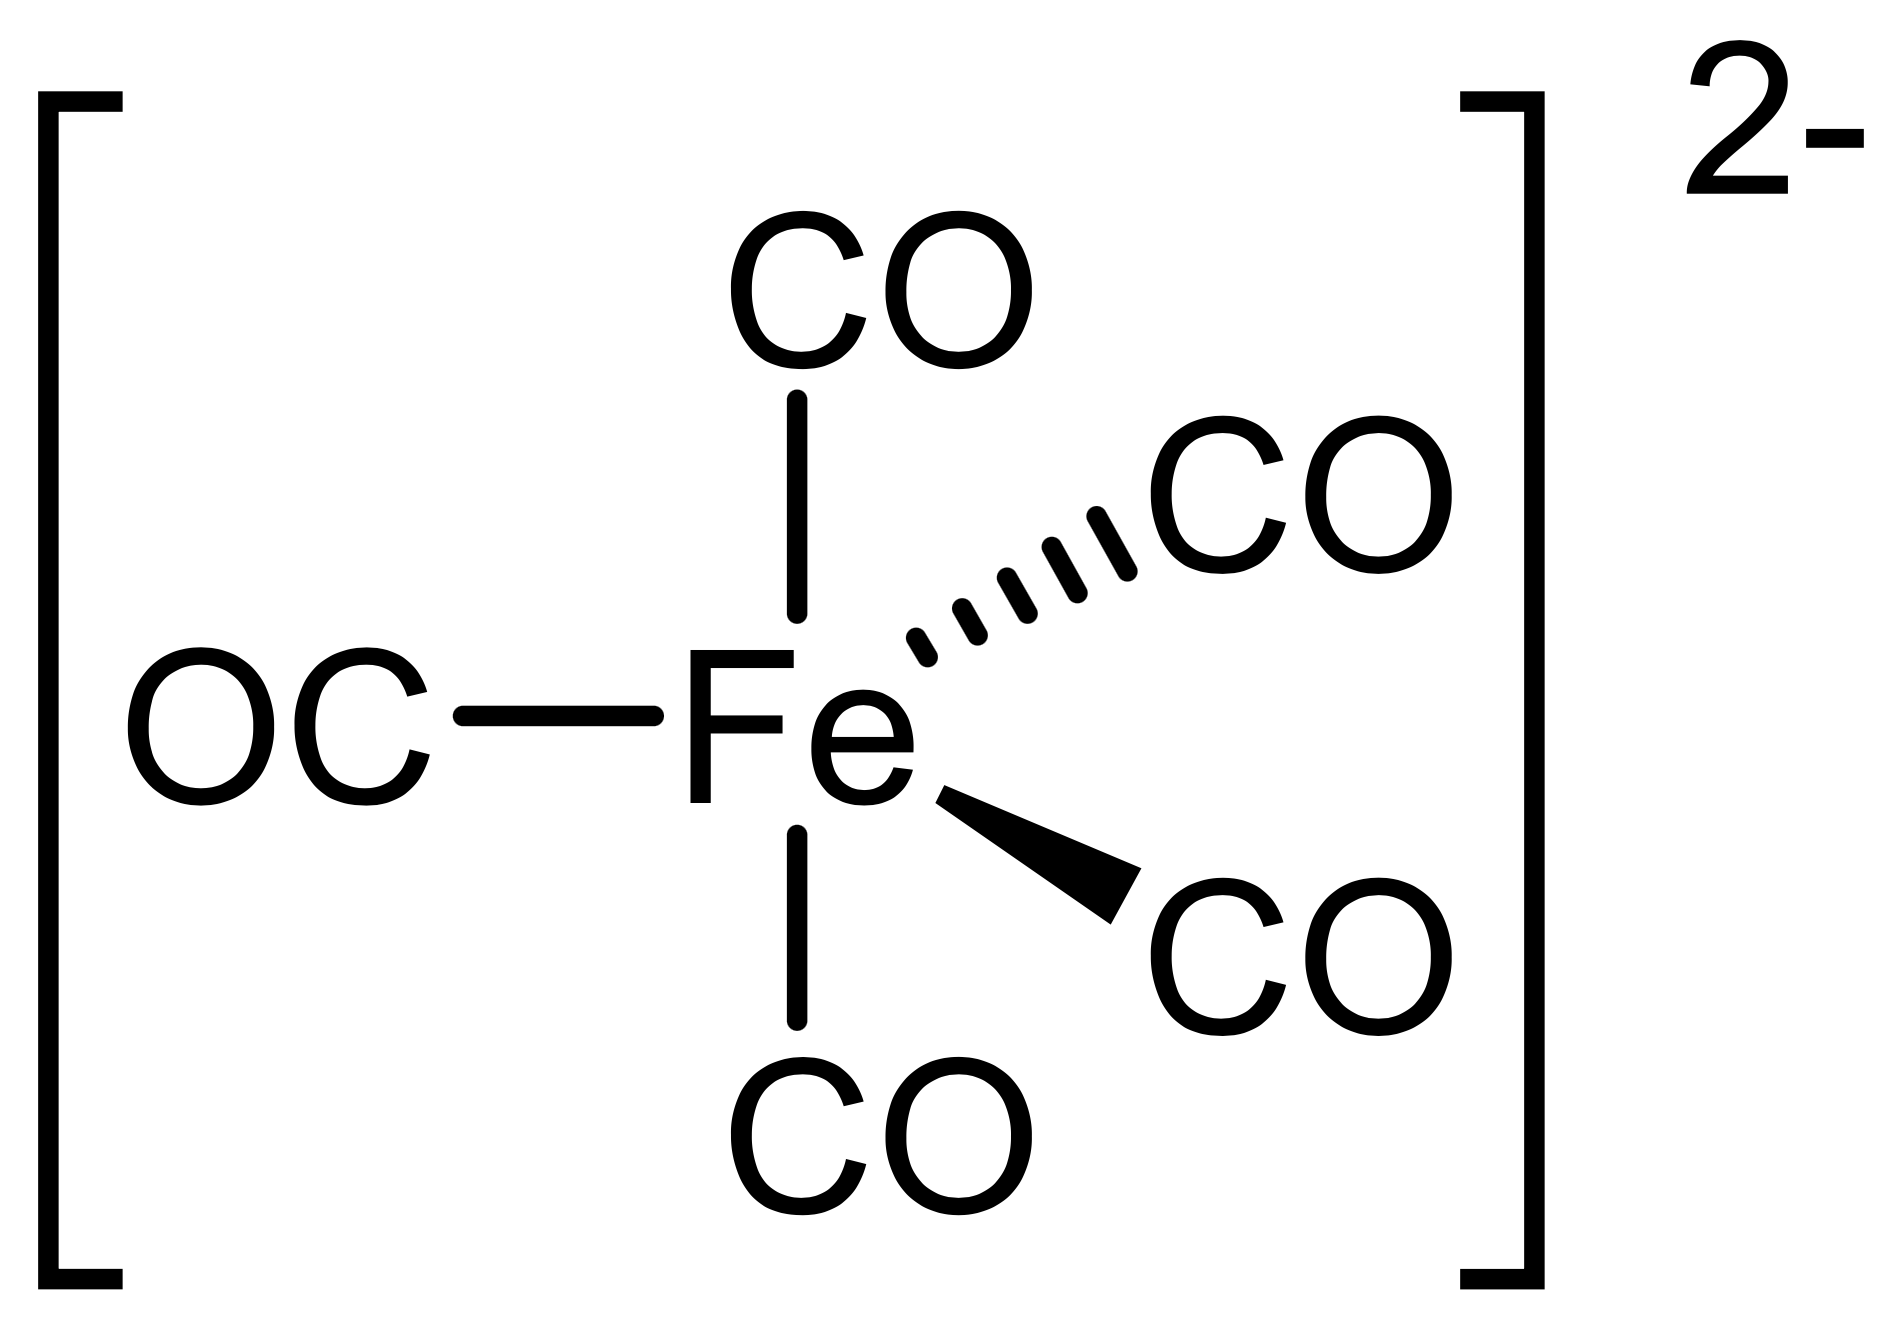
\includegraphics[width=0.25\linewidth]{../ExtFiles/pset1-1-03.png}
        \end{center}
        \begin{proof}[Answer]\leavevmode
            \begin{enumerate}[label={(\roman*)}]
                \item \ce{Fe^2-} (each carbonyl is L-type; the charge is $2-$).
                \item \ce{Fe^2-} is $d^{10}$.
                \item Each carbonyl is a 2-electron donor. Thus, the ligands donate $5\cdot 2=10$ electrons in total. This combined with the above results yields $10+8-(-2)=20$ as the electron count.
            \end{enumerate}
        \end{proof}
        \newpage
        \item ${\color{white}hi}$
        \begin{center}
            % \begin{tikzpicture}
            %     \begin{scope}
            %         \draw (0,0) -- (0.7,-0.2) -- (0.5,-0.5) -- (-0.5,-0.5) -- (-0.7,-0.2) -- cycle;
            %         \draw (0,-0.28) ellipse (0.5cm and 0.15cm);
            %     \end{scope}
            %     \begin{scope}[yshift=-2cm,yscale=-1]
            %         \draw (0,0) -- (0.7,-0.2) -- (0.5,-0.5) -- (-0.5,-0.5) -- (-0.7,-0.2) -- cycle;
            %         \draw (0,-0.28) ellipse (0.5cm and 0.15cm);
            %     \end{scope}
            %     \node at (0,-1) {Fe}
            %         edge (0,-1.7)
            %         edge (0,-0.5)
            %         (0,-0.28) edge (0,-0.43)
            %     ;
            %     \node [anchor=south west,inner sep=0pt] at (0.69,-0.42) {\chemfig{-[:20](=[::60]O)-[::-60]}};
            % \end{tikzpicture}
            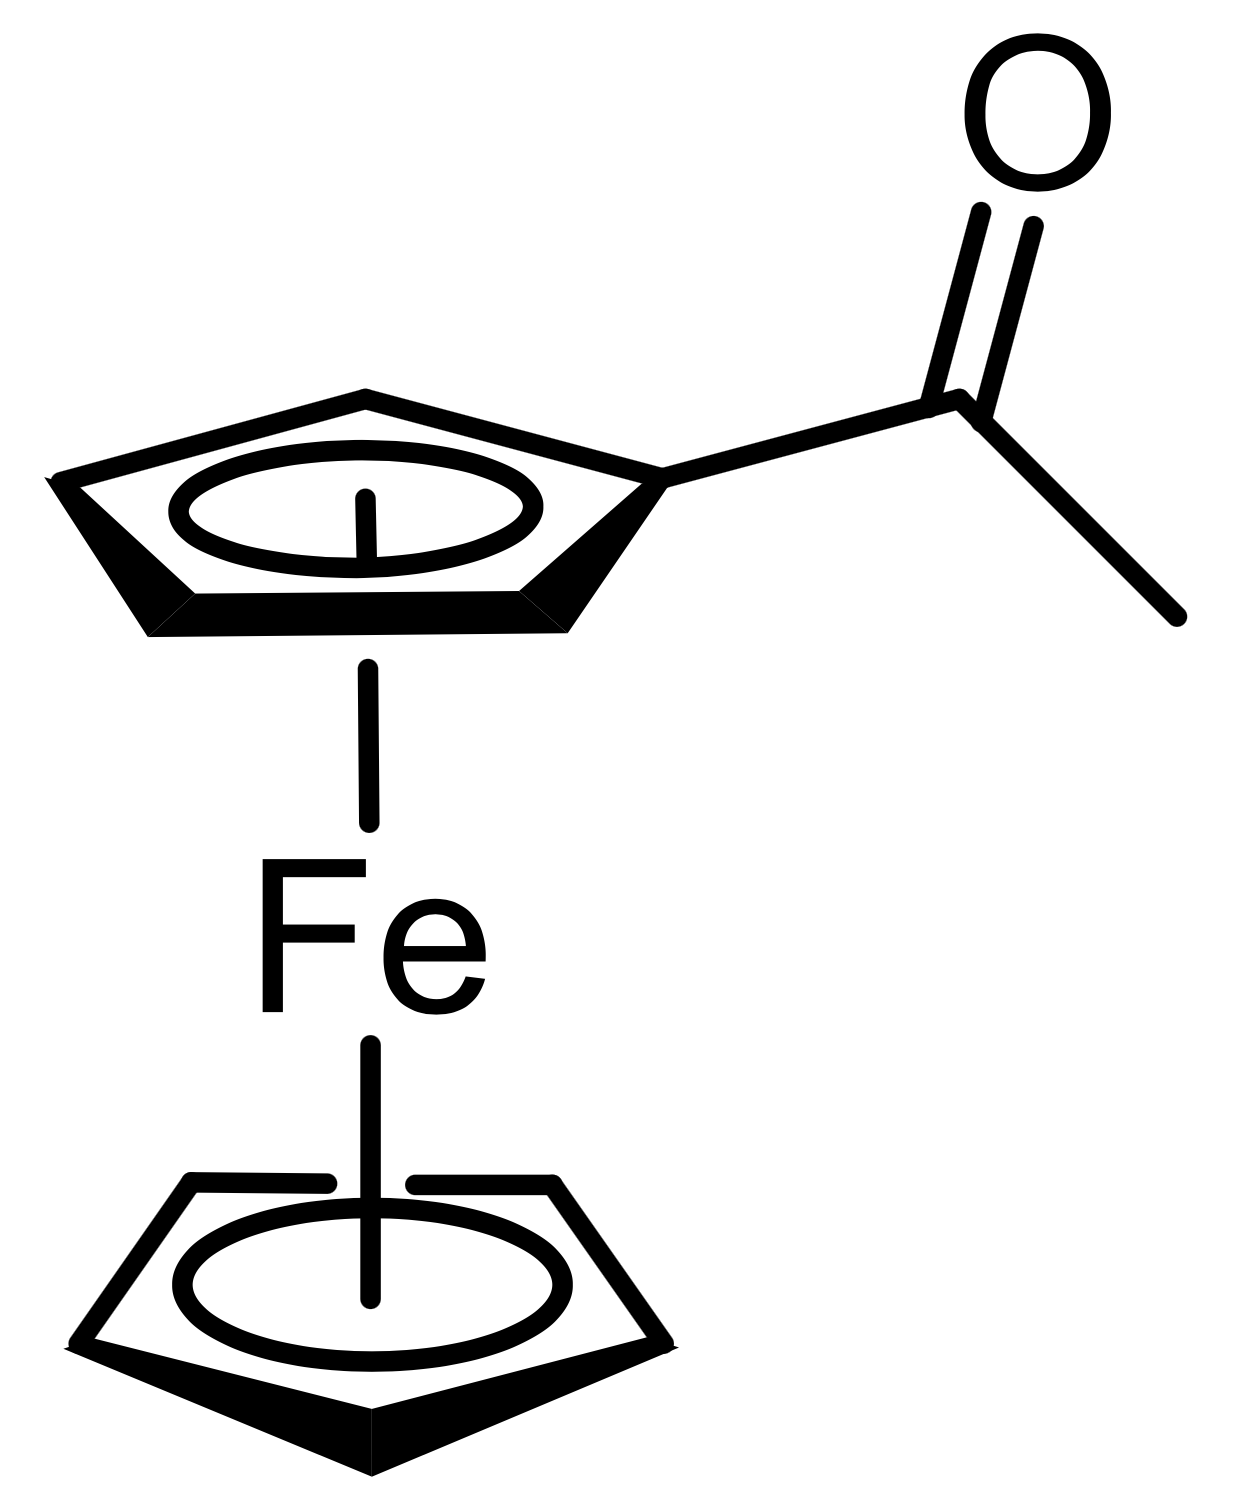
\includegraphics[width=0.18\linewidth]{../ExtFiles/pset1-1-04.png}
        \end{center}
        \begin{proof}[Answer]\leavevmode
            \begin{enumerate}[label={(\roman*)}]
                \item \ce{Fe^2+} (both ligands are X-type).
                \item \ce{Fe^2+} is $d^6$.
                \item Both ligands are 5-electron donors. Thus, the ligands donate $2\cdot 5=10$ electrons in total. This combined with the above results yields $10+8=18$ as the electron count.
            \end{enumerate}
        \end{proof}
        \item ${\color{white}hi}$
        \begin{center}
            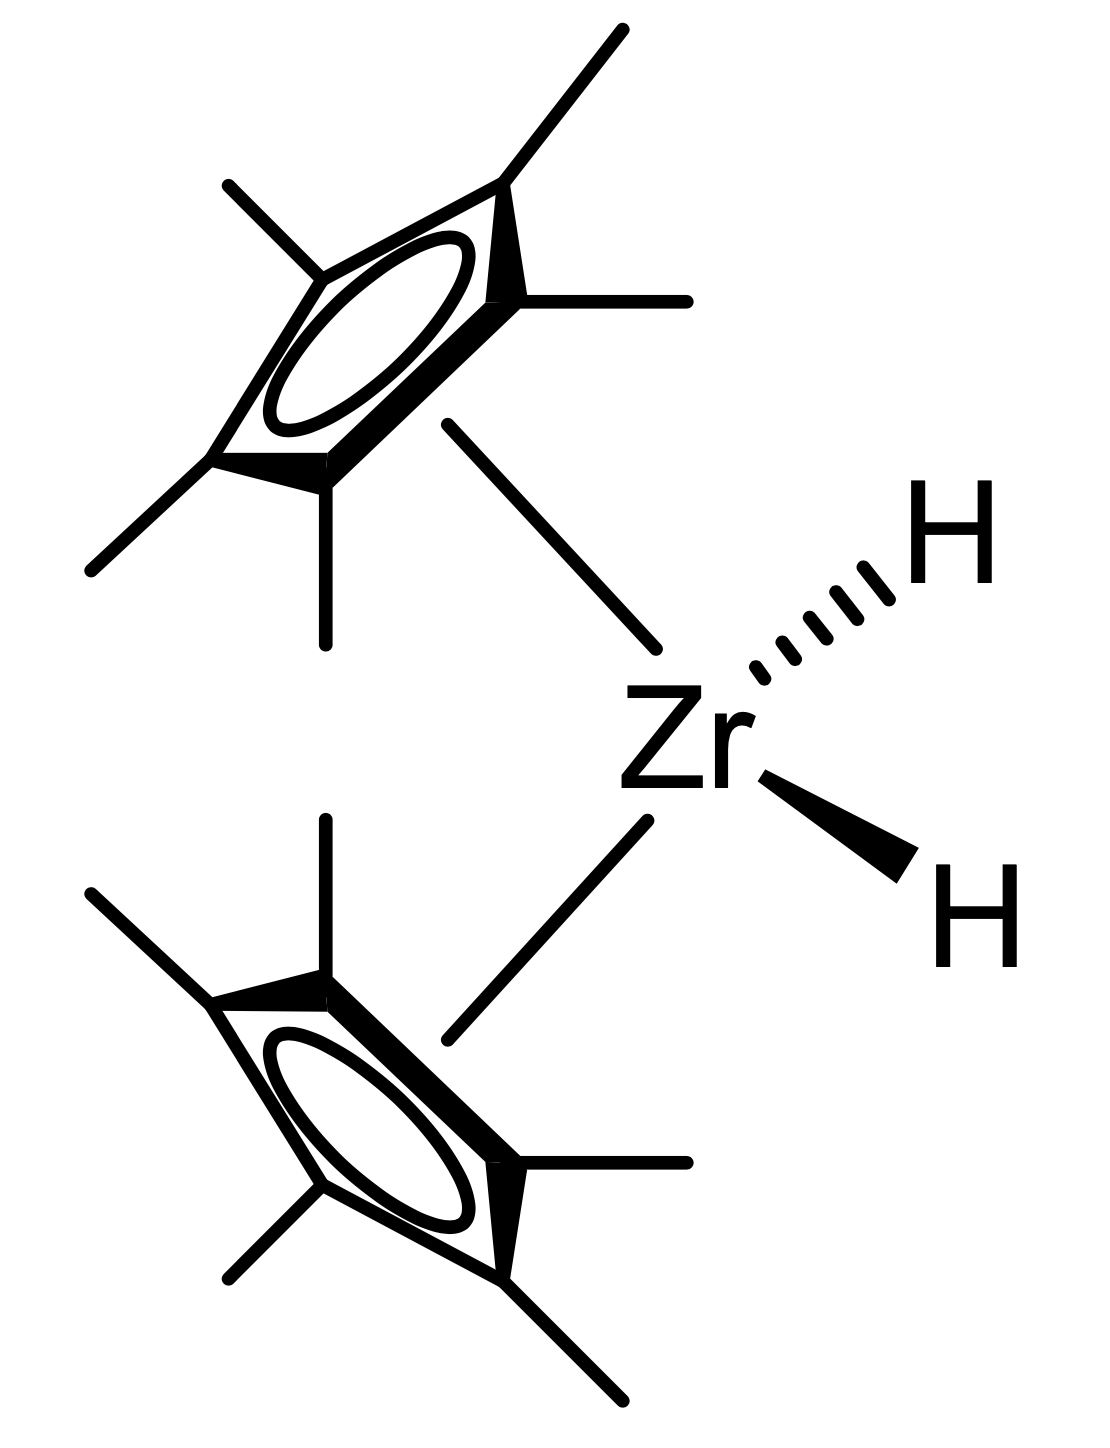
\includegraphics[width=0.2\linewidth]{../ExtFiles/pset1-1-05.png}
        \end{center}
        \begin{proof}[Answer]\leavevmode
            \begin{enumerate}[label={(\roman*)}]
                \item \ce{Zr^4+} (all ligands are X-type).
                \item \ce{Zr^4+} is $d^0$.
                \item Both pentamethylcyclopentadienyl (\ce{Cp^*}) groups are 5-electron donors, and both hydrogens are 1-electron donors. Thus, the ligands donate $2\cdot 5+2\cdot 1=12$ electrons in total. This combined with the above results yields $12+4=16$ as the electron count.
            \end{enumerate}
        \end{proof}
        \item ${\color{white}hi}$
        \begin{center}
            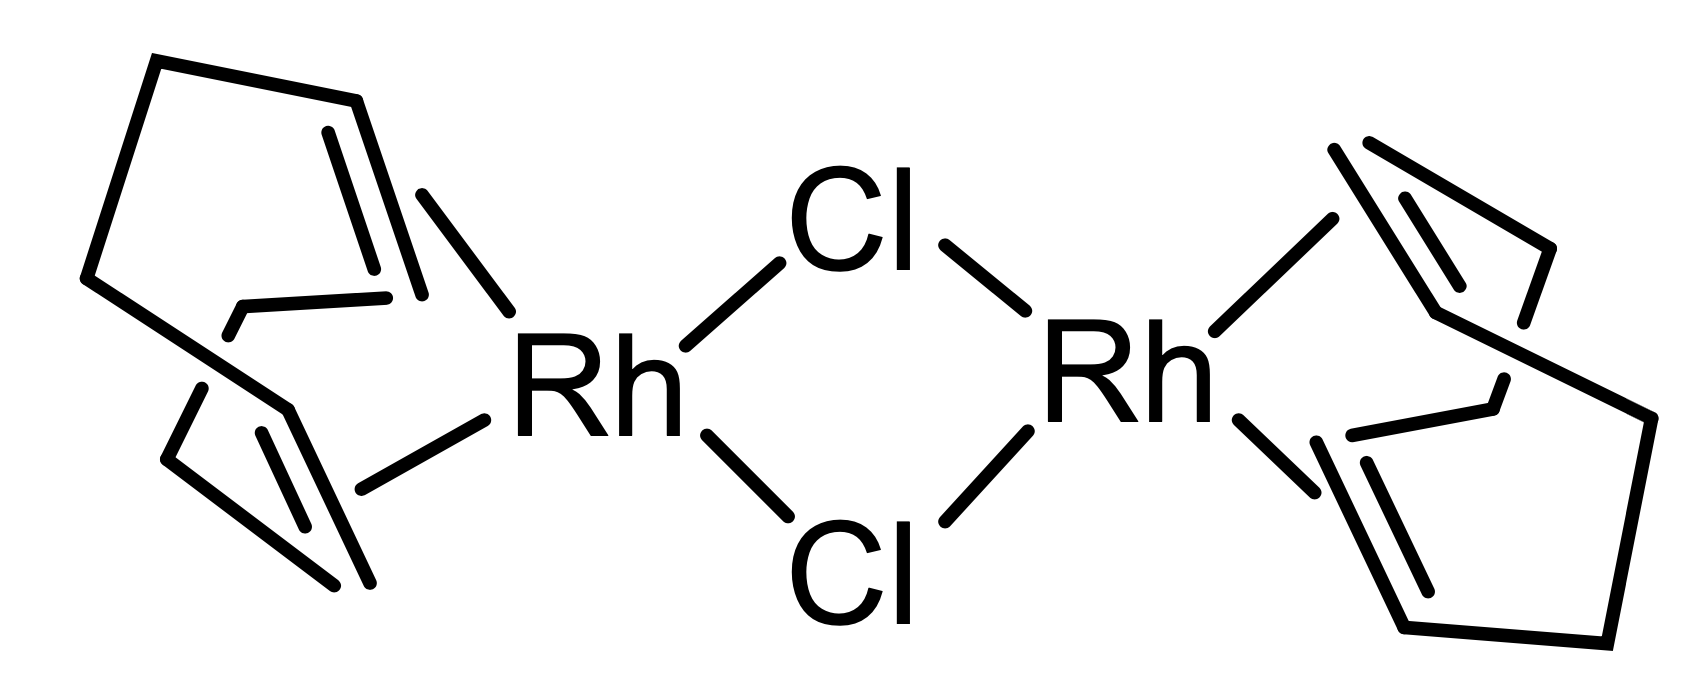
\includegraphics[width=0.3\linewidth]{../ExtFiles/pset1-1-06.png}
        \end{center}
        \begin{proof}[Answer]\leavevmode
            \begin{enumerate}[label={(\roman*)}]
                \item Both metals are \ce{Rh^+} (both cycloocta-1,5-dienyl (COD) groups are \ce{L2}-type; both bridging chlorines are LX-type [they can be thought of as bonding covalently to one rhodium and datively to the other, so when the bonds are cleaved, each chlorine steals one covalent electron from a rhodium and reclaims its two dative electrons]).
                \item \ce{Rh^+} is $d^8$.
                \item Both COD groups are 4-electron donors, and both bridging chlorines are 3-electron donors. Thus, the ligands donate $2\cdot 4+2\cdot 3=14$ electrons in total. This combined with the above results yields $\frac{14+2\cdot 9}{2}=16$ as the electron count at each rhodium. It follows that there should be $\frac{36-2\cdot 16}{2}=2$ \ce{Rh-Rh} bonds.
            \end{enumerate}
        \end{proof}
        \newpage
        \item ${\color{white}hi}$
        \begin{center}
            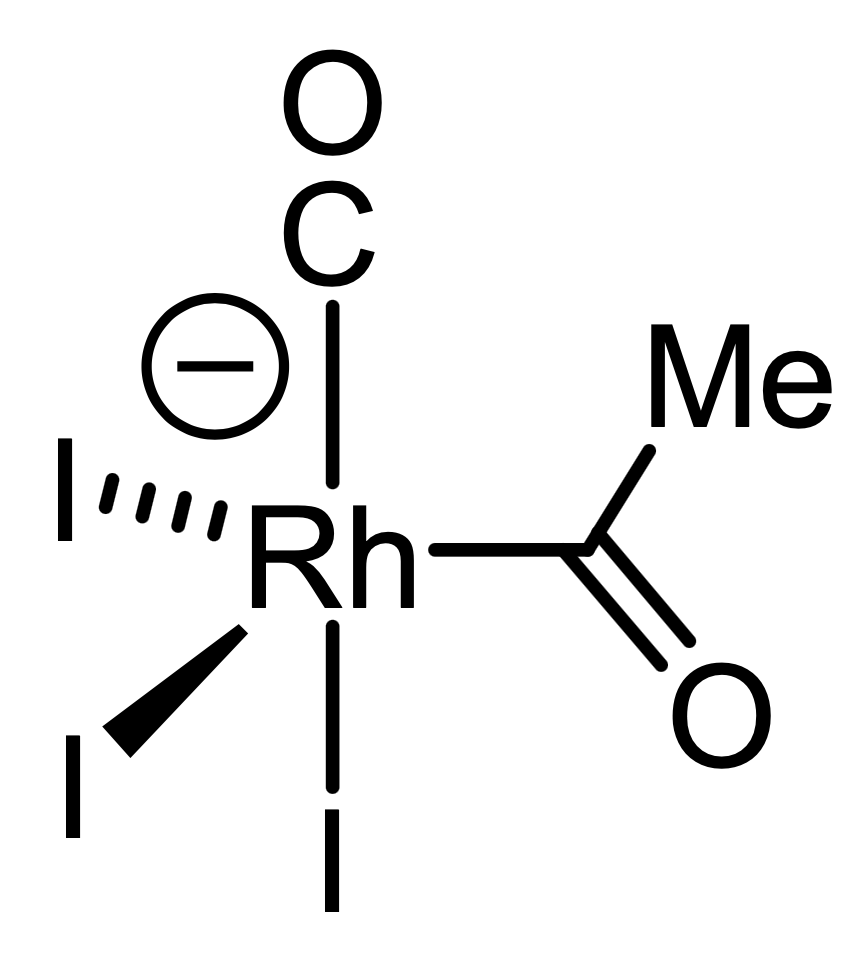
\includegraphics[width=0.16\linewidth]{../ExtFiles/pset1-1-07.png}
        \end{center}
        \begin{proof}[Answer]\leavevmode
            \begin{enumerate}[label={(\roman*)}]
                \item \ce{Rh^3+} (the carbonyl is L-type; each iodide is X-type; the other ligand is X-type; the charge is $1-$).
                \item \ce{Rh^3+} is $d^6$.
                \item The carbonyl is a 2-electron donor, each iodide is a 1-electron donor, and the other ligand is a 1-electron donor. Thus, the ligands donate $1\cdot 2+3\cdot 1+1\cdot 1=6$ electrons in total. This combined with the above results yields $6+9-(-1)=16$ as the electron count.
            \end{enumerate}
        \end{proof}
        \item ${\color{white}hi}$
        \begin{center}
            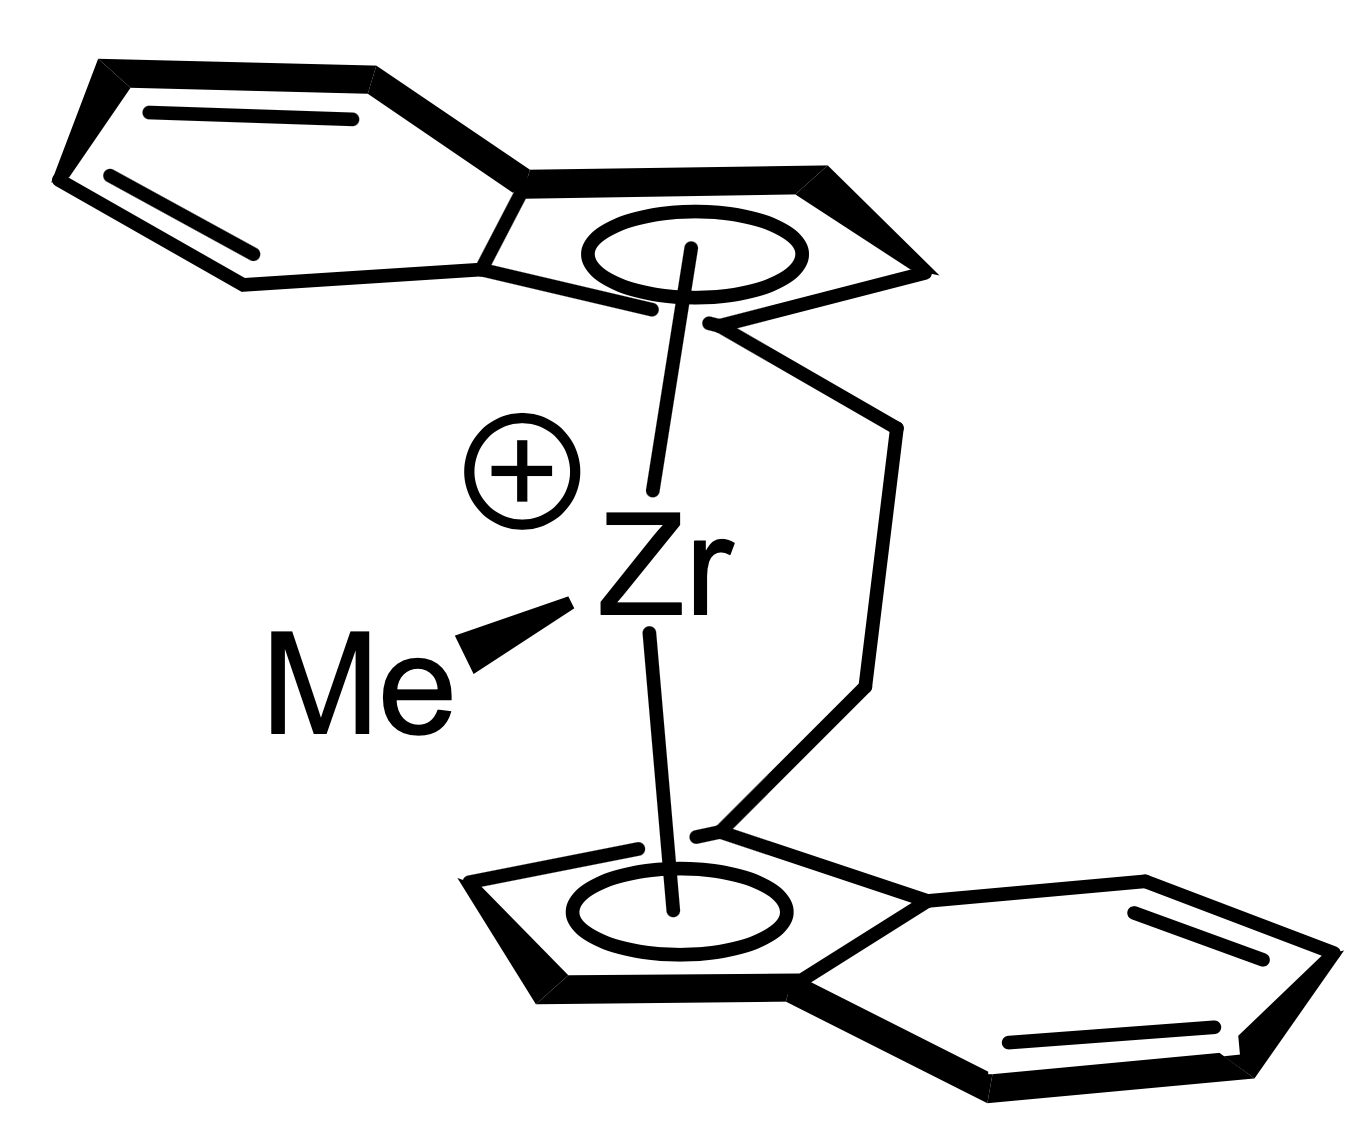
\includegraphics[width=0.25\linewidth]{../ExtFiles/pset1-1-08.png}
        \end{center}
        \begin{proof}[Answer]\leavevmode
            \begin{enumerate}[label={(\roman*)}]
                \item \ce{Zr^4+} (the methyl is X-type; the other ligand is \ce{X2}-type; the charge is $1+$).
                \item \ce{Zr^4+} is $d^0$.
                \item The methyl is a 1-electron donor, and the other ligand is a 10-electron donor. Thus, the ligands donate $1\cdot 1+1\cdot 10=11$ electrons in total. This combined with the above results yields $11+4-1=14$ as the electron count.
            \end{enumerate}
        \end{proof}
        \item ${\color{white}hi}$
        \begin{center}
            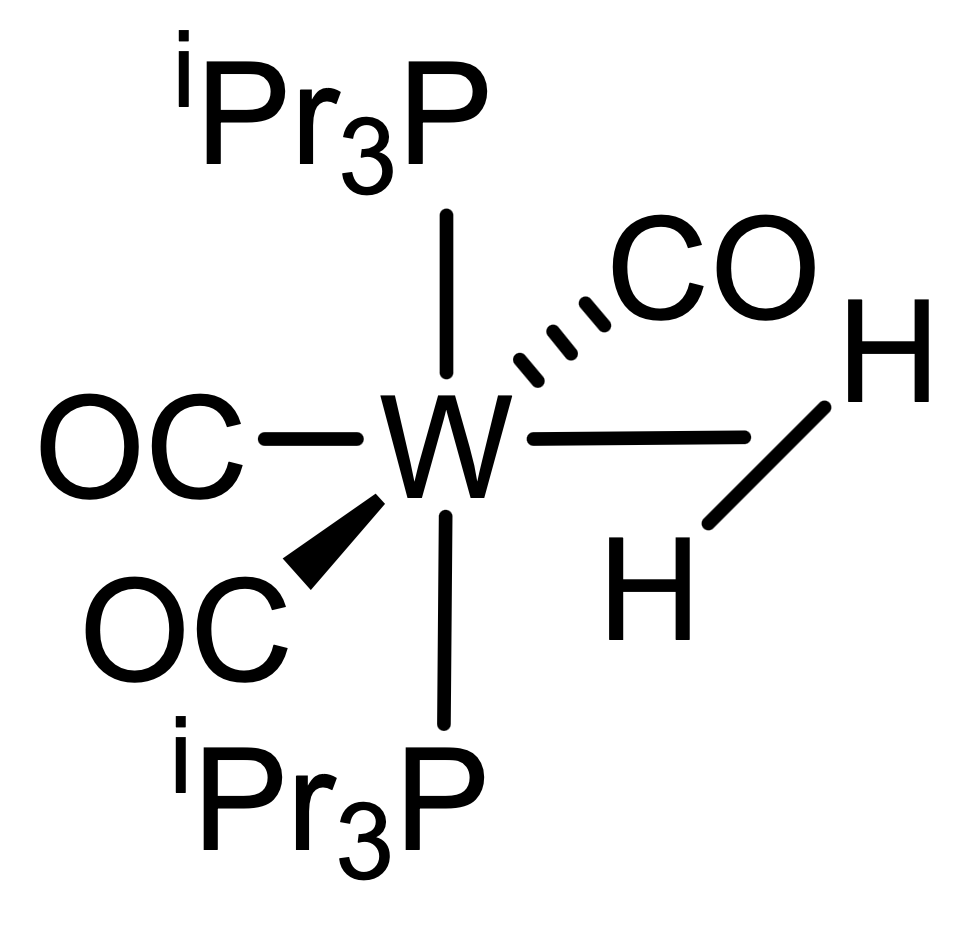
\includegraphics[width=0.18\linewidth]{../ExtFiles/pset1-1-09.png}
        \end{center}
        \begin{proof}[Answer]\leavevmode
            \begin{enumerate}[label={(\roman*)}]
                \item \ce{W^0} (each carbonyl is L-type; both phosphines are L-type; the other ligand is L-type).
                \item \ce{W^0} is $d^6$.
                \item Each carbonyl is a 2-electron donor, both phosphines are 2-electron donors, and the other ligand is a 2-electron donor. Thus, the ligands donate $3\cdot 2+2\cdot 2+1\cdot 2=12$ electrons in total. This combined with the above results yields $12+6=18$ as the electron count.
            \end{enumerate}
        \end{proof}
        \newpage
        \item ${\color{white}hi}$
        \begin{center}
            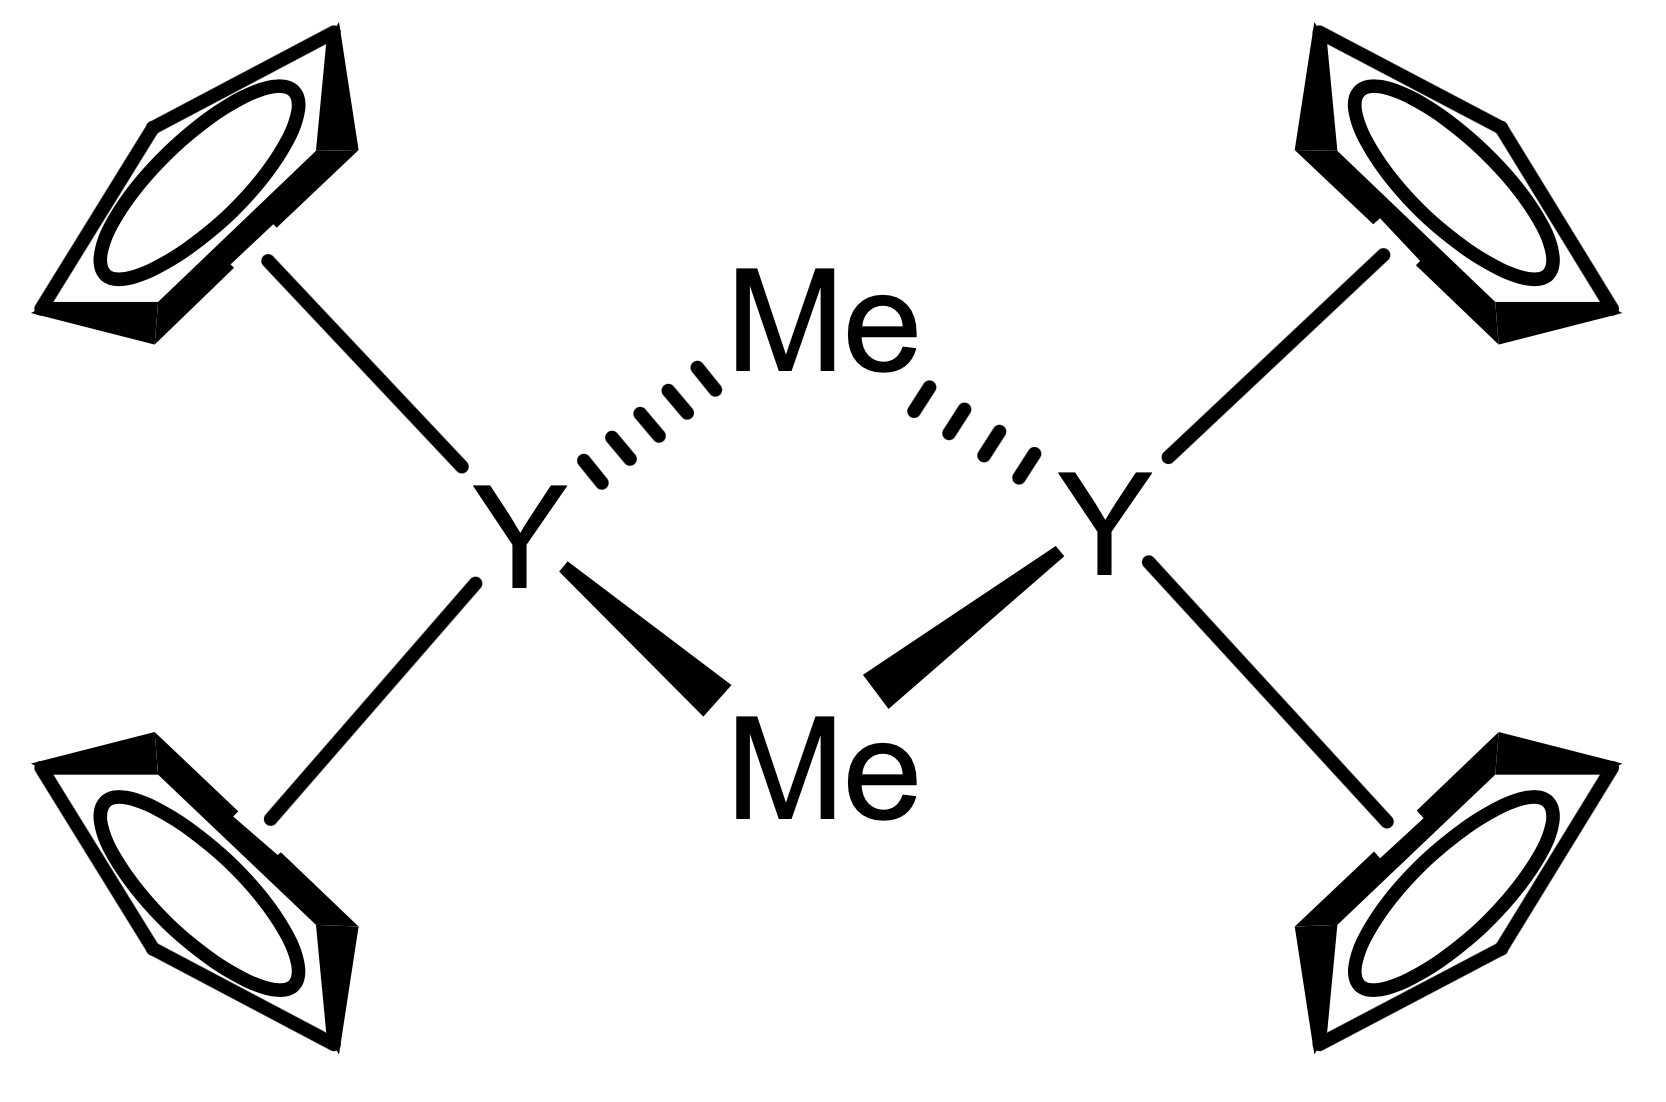
\includegraphics[width=0.32\linewidth]{../ExtFiles/pset1-1-10.png}
        \end{center}
        \begin{proof}[Answer]\leavevmode
            \begin{enumerate}[label={(\roman*)}]
                \item \ce{Y^3+} (each Cp is X-type; each bridging methyl is LX-type).
                \item \ce{Y^3+} is $d^0$.
                \item Each Cp is a 5-electron donor, and each methyl is a 3-electron donor. Thus, the ligands donate $4\cdot 5+2\cdot 3=26$ electrons in total. This combined with the above results yields $\frac{26+2\cdot 3}{2}=16$ as the electron count at each yttrium. It follows that there should be $\frac{36-2\cdot 16}{2}=2$ \ce{Y-Y} bonds.
            \end{enumerate}
        \end{proof}
        \item ${\color{white}hi}$
        \begin{center}
            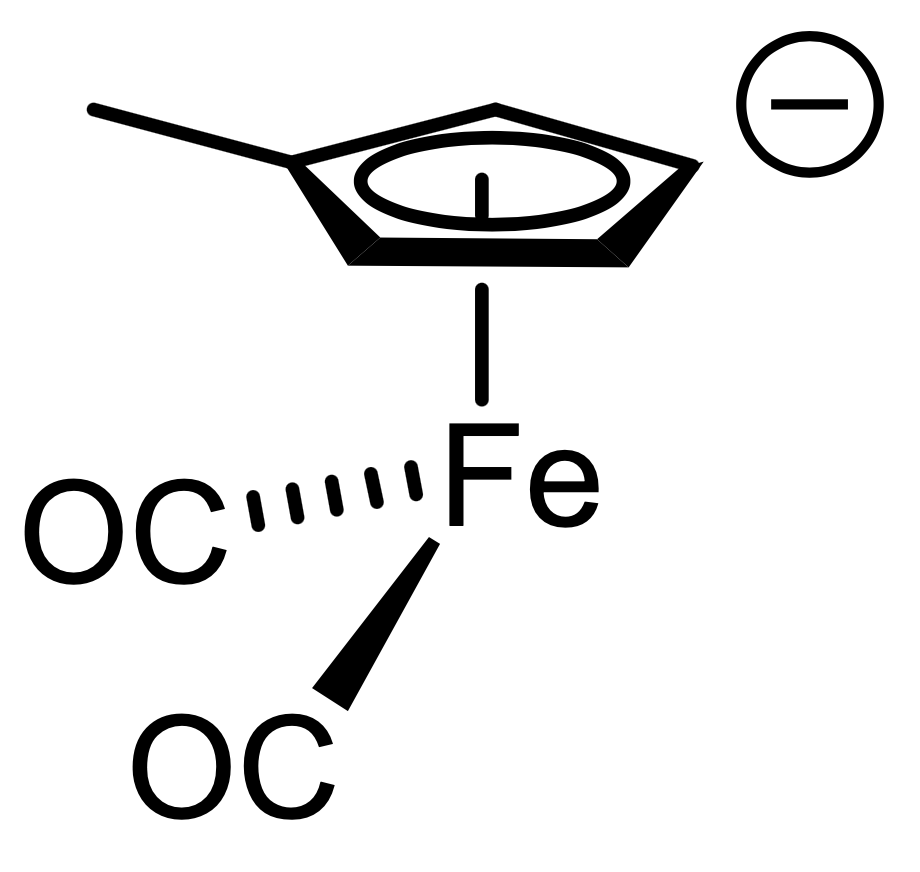
\includegraphics[width=0.18\linewidth]{../ExtFiles/pset1-1-11.png}
        \end{center}
        \begin{proof}[Answer]\leavevmode
            \begin{enumerate}[label={(\roman*)}]
                \item \ce{Fe^0} (both carbonyls are L-type; the other ligand is X-type; the charge is $1-$).
                \item \ce{Fe^0} is $d^8$.
                \item Both carbonyls are 2-electron donors, and the methylcyclopentadienyl group is a 5-electron donor. Thus, the ligands donate $2\cdot 2+1\cdot 5=9$ electrons in total. This combined with the above results yields $9+8-(-1)=18$ as the electron count.
            \end{enumerate}
        \end{proof}
        \item ${\color{white}hi}$
        \begin{center}
            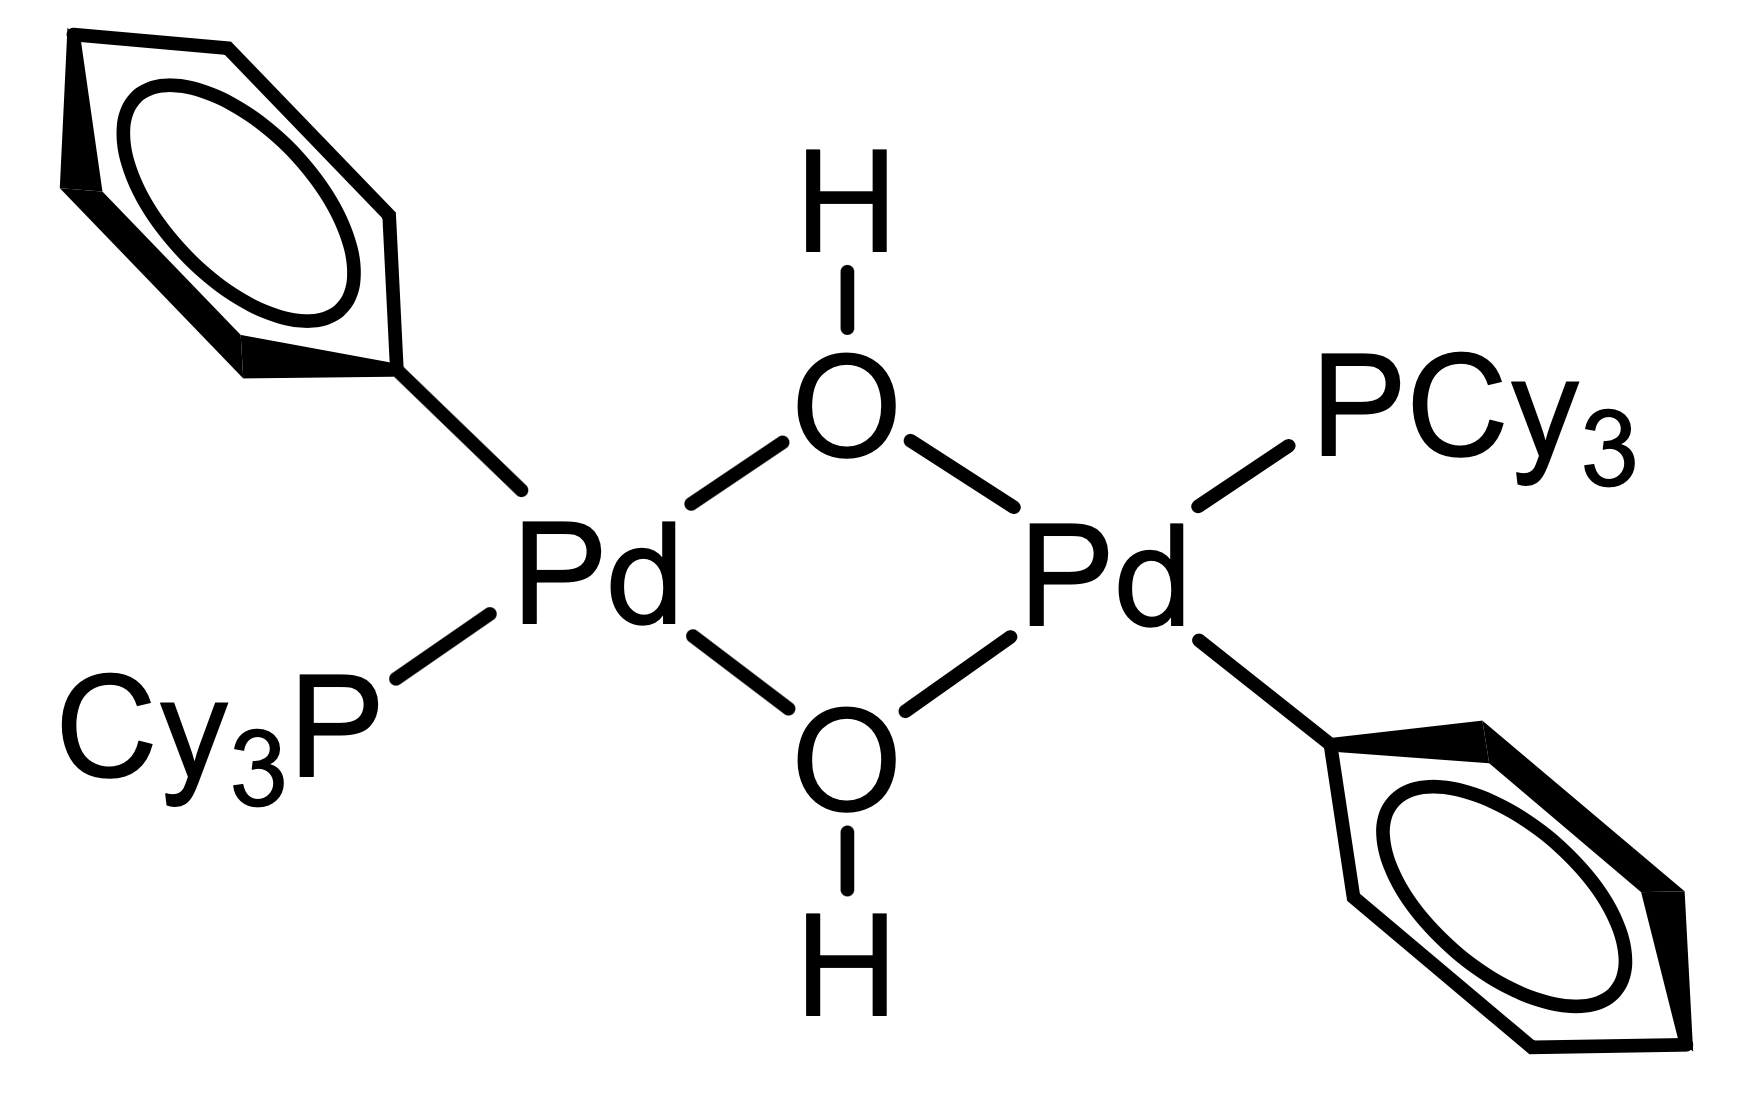
\includegraphics[width=0.34\linewidth]{../ExtFiles/pset1-1-12.png}
        \end{center}
        \begin{proof}[Answer]\leavevmode
            \begin{enumerate}[label={(\roman*)}]
                \item \ce{Pd^2+} (both benzenes are X-type; both phosphines are L-type; both bridging hydroxides are LX-type).
                \item \ce{Pd^2+} is $d^8$.
                \item Both benzenes are 1-electron donors, both phosphines are 2-electron donors, and both bridging hydroxides are 3-electron donors. Thus, the ligands donate $2\cdot 1+2\cdot 2+2\cdot 3=12$ electrons in total. This combined with the above results yields $\frac{12+2\cdot 10}{2}=16$ as the electron count at each palladium. It follows that there should be $\frac{36-2\cdot 16}{2}=2$ \ce{Pd-Pd} bonds.
            \end{enumerate}
        \end{proof}
        \newpage
        \item ${\color{white}hi}$
        \begin{center}
            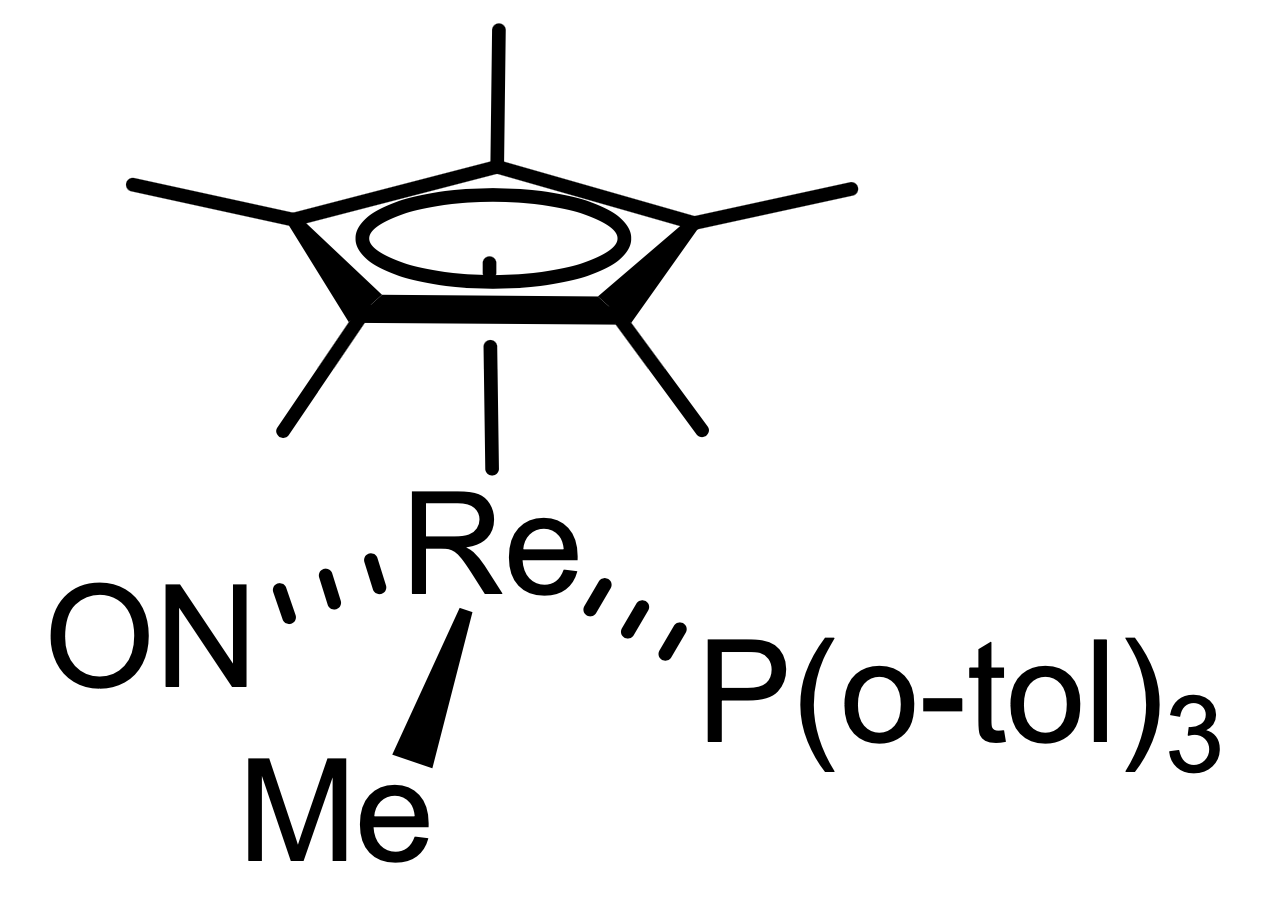
\includegraphics[width=0.24\linewidth]{../ExtFiles/pset1-1-13.png}
        \end{center}
        \begin{proof}[Answer]\leavevmode
            \begin{enumerate}[label={(\roman*)}]
                \item \ce{Re^+} (the [linear] nitrosyl group is L-type but takes on a positive charge during bond cleavage; the methyl group is X-type; the phosphine is L-type; the \ce{Cp^*} group is X-type).
                \item \ce{Re^+} is $d^6$.
                \item The nitrosyl group is a 3-electron donor (assuming it bonds linearly), the methyl group is a 1-electron donor, the phosphine is a 2-electron donor, and the \ce{Cp^*} is a 5-electron donor. Thus, the ligands donate $1\cdot 3+1\cdot 1+1\cdot 2+1\cdot 5=11$ electrons in total. This combined with the above results yields $11+7=18$ as the electron count.
            \end{enumerate}
        \end{proof}
        \item ${\color{white}hi}$
        \begin{center}
            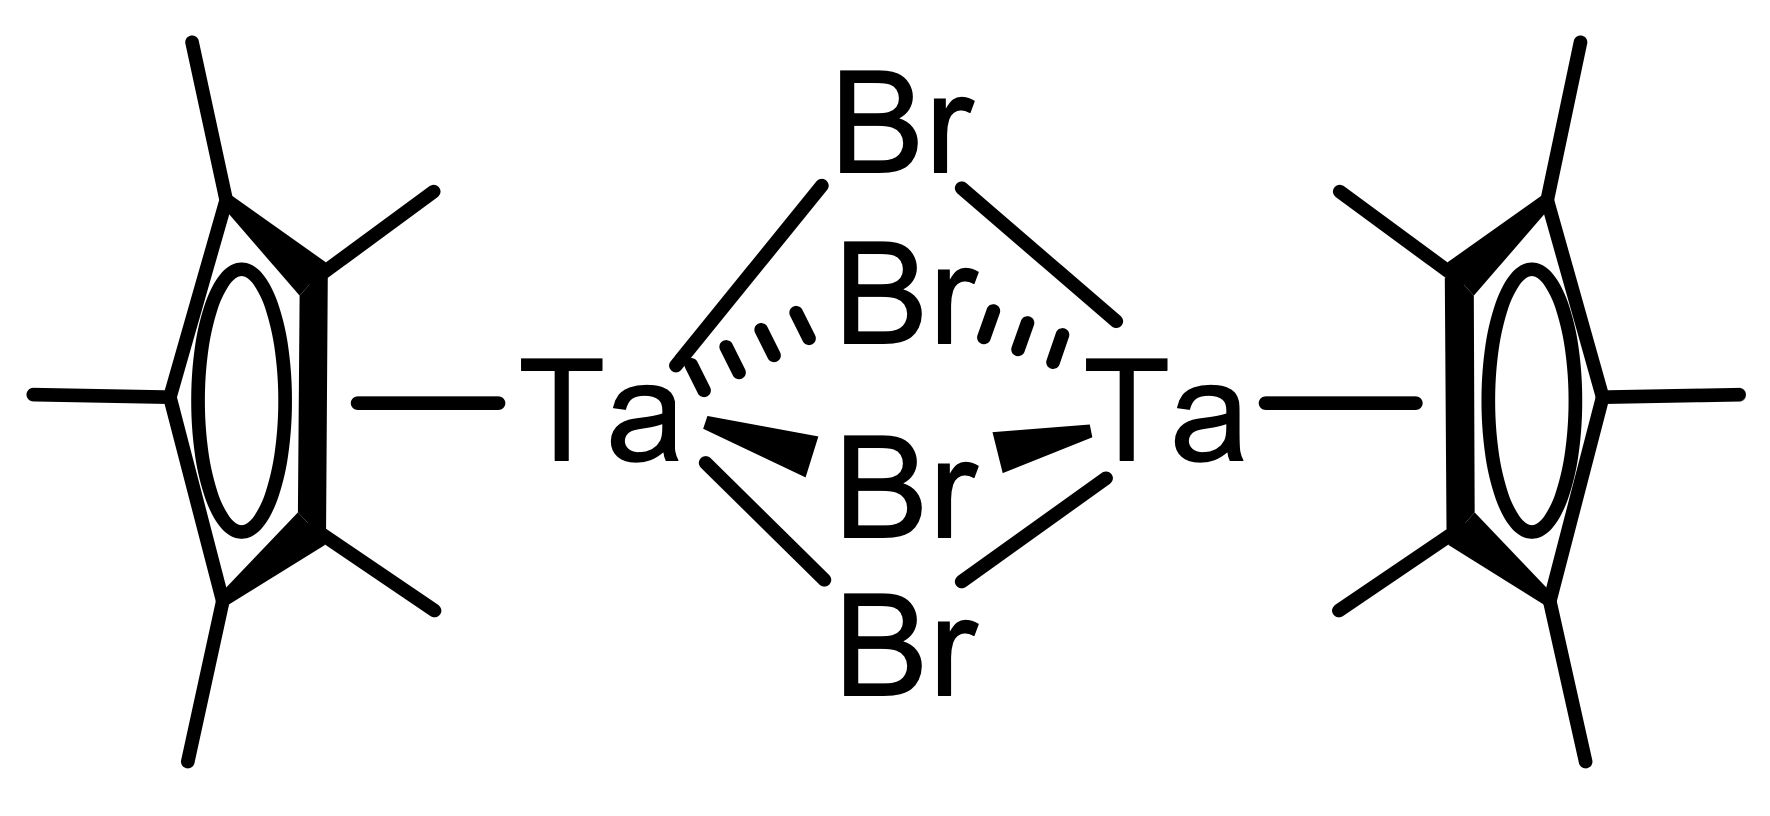
\includegraphics[width=0.34\linewidth]{../ExtFiles/pset1-1-14.png}
        \end{center}
        \begin{proof}[Answer]\leavevmode
            \begin{enumerate}[label={(\roman*)}]
                \item \ce{Ta^3+} (both \ce{Cp^*} groups are L-type; each bridging bromine is LX-type).
                \item \ce{Ta^3+} is $d^2$.
                \item Both \ce{Cp^*} groups are 5-electron donors, and each bridging bromine is a 3-electron donor. Thus, the ligands donate $2\cdot 5+4\cdot 3=22$ electrons in total. This combined with the above results yields $\frac{22+2\cdot 5}{2}=16$ as the electron count at each tantalum. It follows that there should be $\frac{36-2\cdot 16}{2}=2$ \ce{Ta-Ta} bonds.
            \end{enumerate}
        \end{proof}
        \item ${\color{white}hi}$
        \begin{center}
            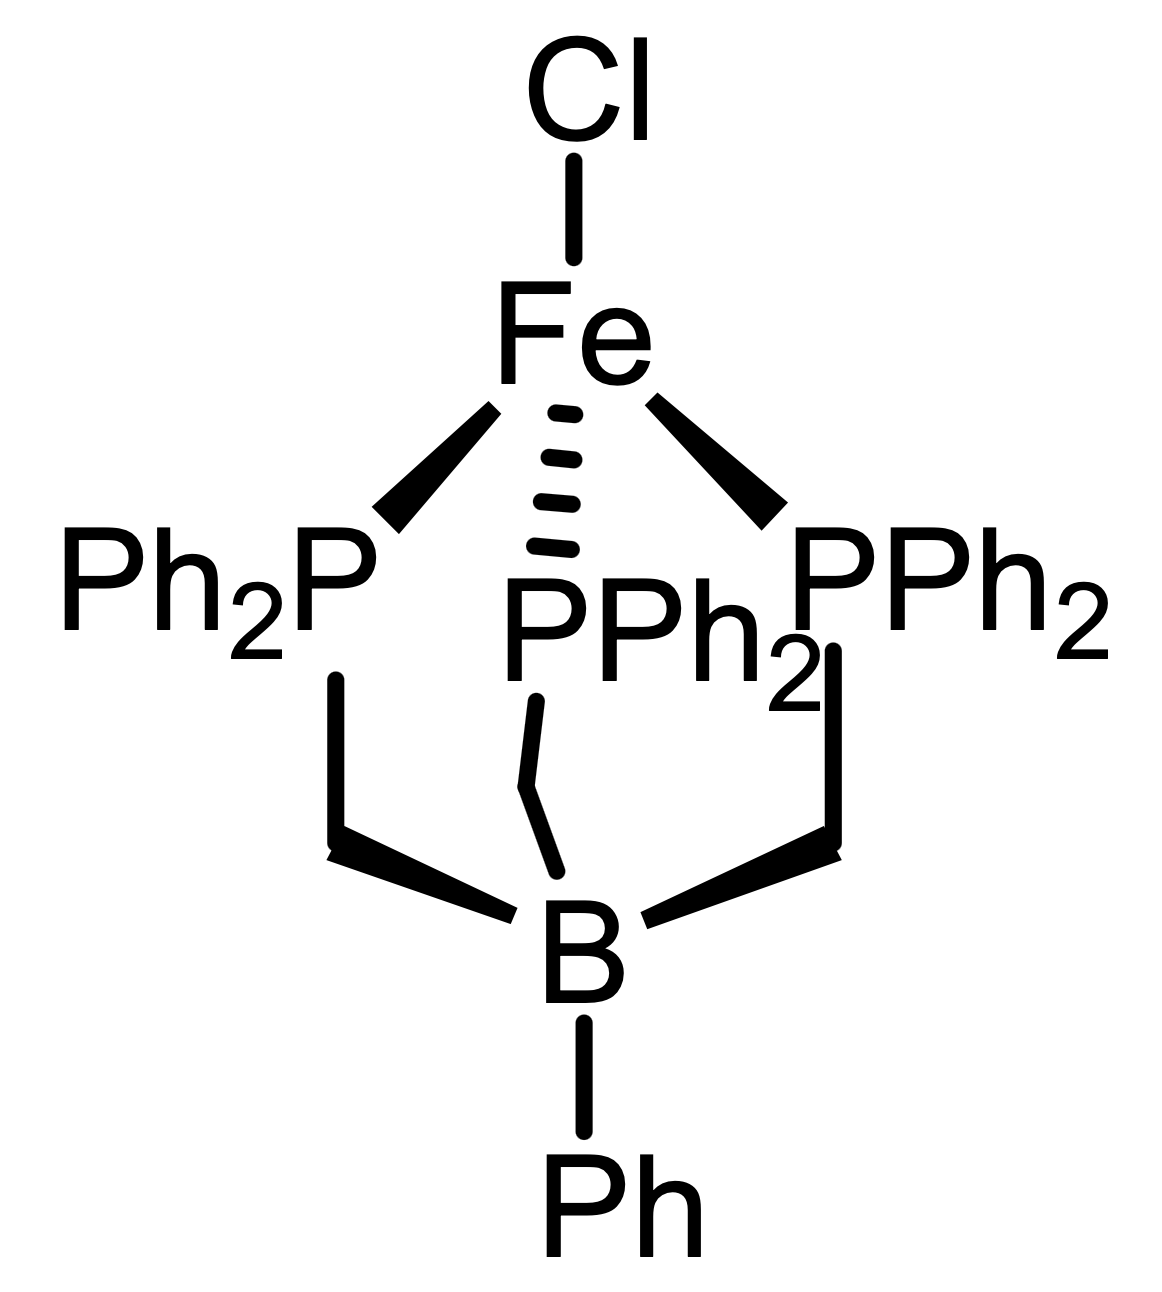
\includegraphics[width=0.22\linewidth]{../ExtFiles/pset1-1-15.png}
        \end{center}
        \begin{proof}[Answer]\leavevmode
            \begin{enumerate}[label={(\roman*)}]
                \item \ce{Fe^2+} (the chloride is X-type; the other ligand is \ce{L3}-type but carries a negative formal charge).
                \item \ce{Fe^2+} is $d^6$.
                \item The chlorine is a 1-electron donor, and the other ligand is a 5-electron donor (3 dative bonds minus a single negative formal charge on the boron). Thus, the ligands donate $1\cdot 1+1\cdot 5=6$ electrons in total. This combined with the above results yields $6+8=14$ as the electron count.
            \end{enumerate}
        \end{proof}
        \newpage
        \item ${\color{white}hi}$
        \begin{center}
            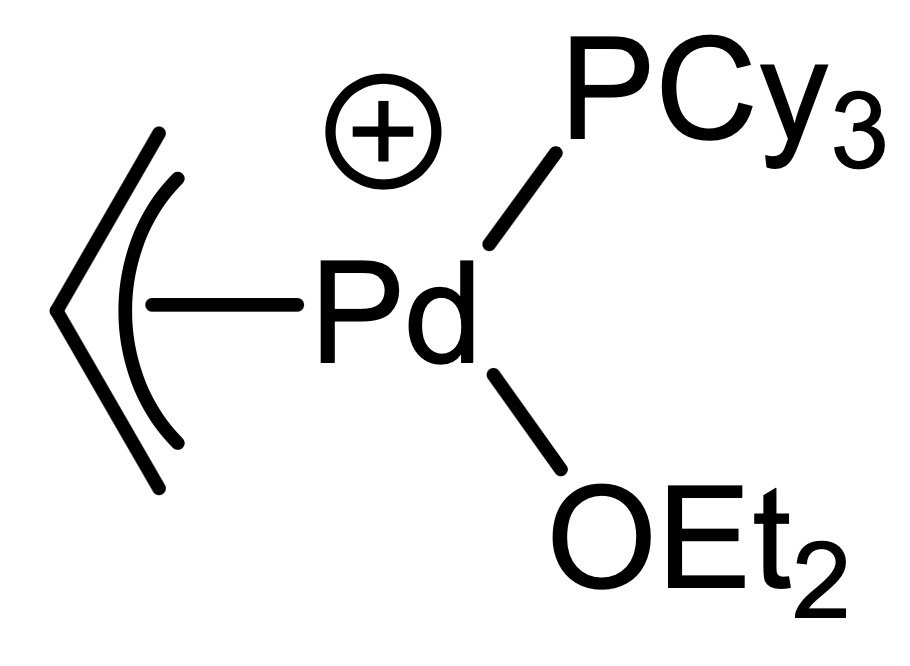
\includegraphics[width=0.18\linewidth]{../ExtFiles/pset1-1-16.png}
        \end{center}
        \begin{proof}[Answer]\leavevmode
            \begin{enumerate}[label={(\roman*)}]
                \item \ce{Pd^0} (the phosphine is L-type; the ether is L-type; the other ligand is L-type but takes on a positive charge during bond cleavage; the charge is $1+$).
                \item \ce{Pd^0} is $d^{10}$.
                \item The phosphine is a 2-electron donor, the ether is a 2-electron donor, and the other ligand is a 3-electron donor. Thus, the ligands donate $1\cdot 2+1\cdot 2+1\cdot 3=7$ electrons in total. This combined with the above result yields $7+10-1=16$ as the electron count.
            \end{enumerate}
        \end{proof}
        \item ${\color{white}hi}$
        \begin{center}
            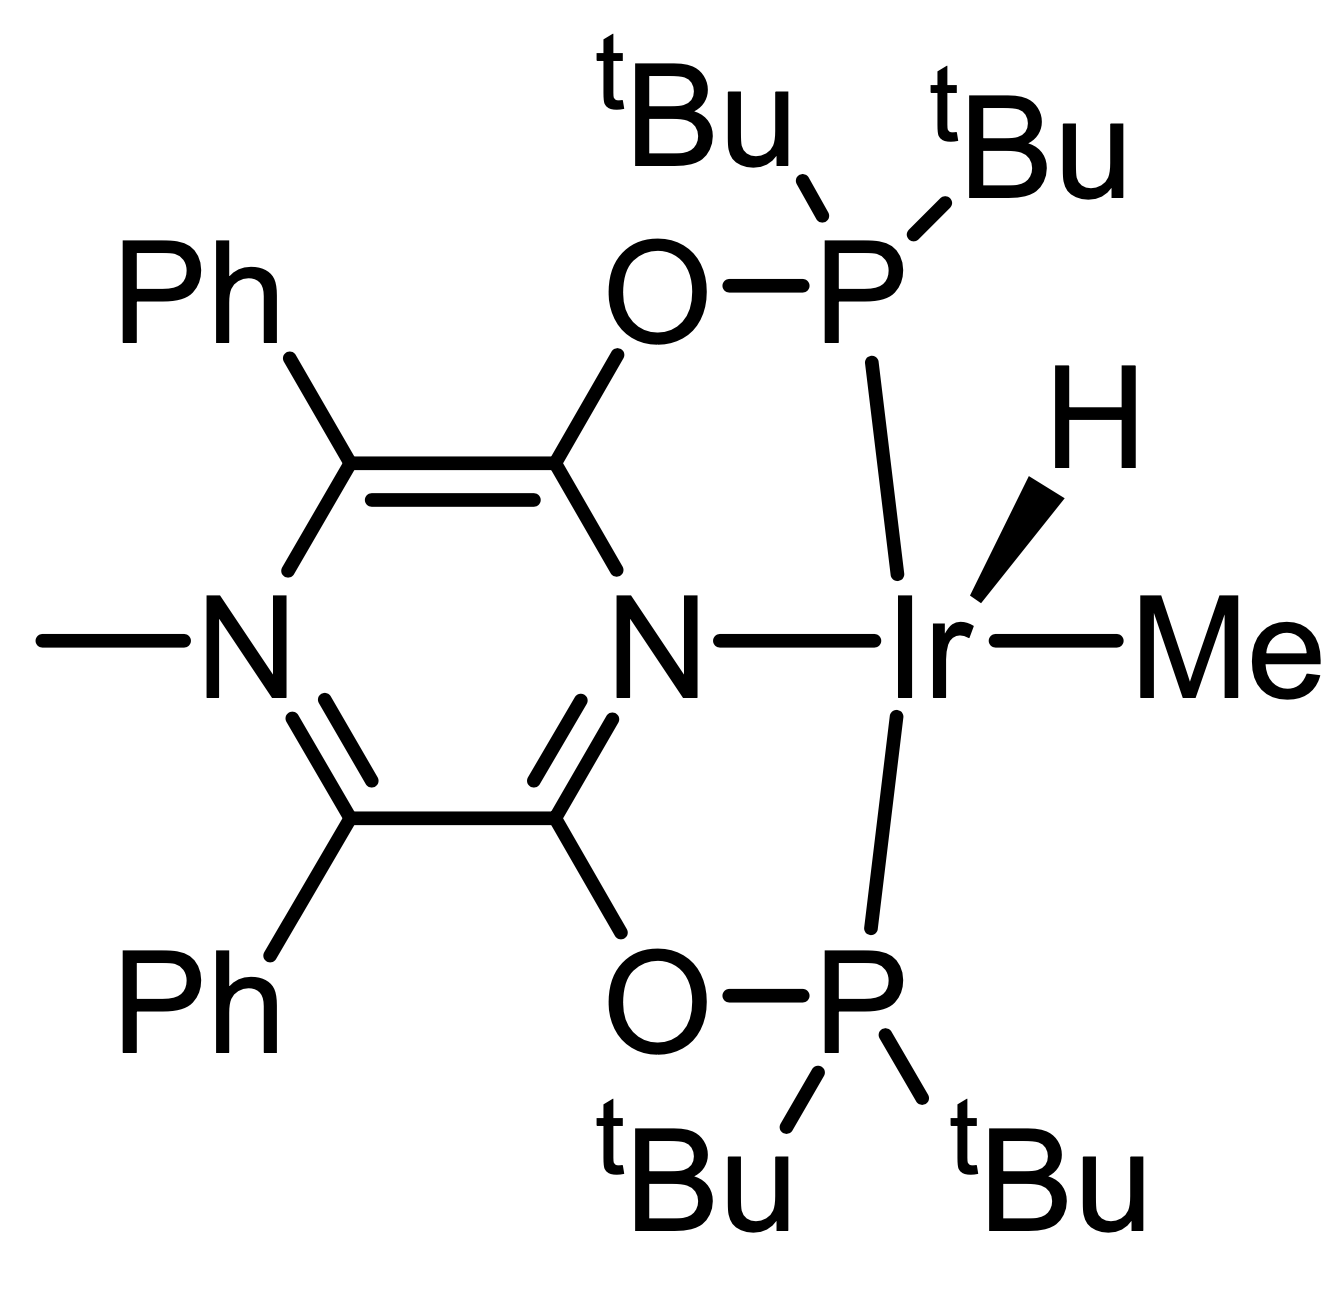
\includegraphics[width=0.24\linewidth]{../ExtFiles/pset1-1-17.png}
        \end{center}
        \begin{proof}[Answer]\leavevmode
            \begin{enumerate}[label={(\roman*)}]
                \item \ce{Ir^2+} (the methyl is X-type; the hydride is X-type; the other ligand is \ce{L3}-type).
                \item \ce{Ir^2+} is $d^7$.
                \item The methyl group is a 1-electron donor, the hydrogen is a 1-electron donor, and the other ligand is a 7-electron donor (3 dative bonds plus a single positive formal charge on the leftmost nitrogen in the above picture). Thus, the ligands donate $1\cdot 1+1\cdot 1+1\cdot 7=9$ electrons in total. This combined with the above result yields $9+9=18$ as the electron count.
            \end{enumerate}
        \end{proof}
        \item ${\color{white}hi}$
        \begin{center}
            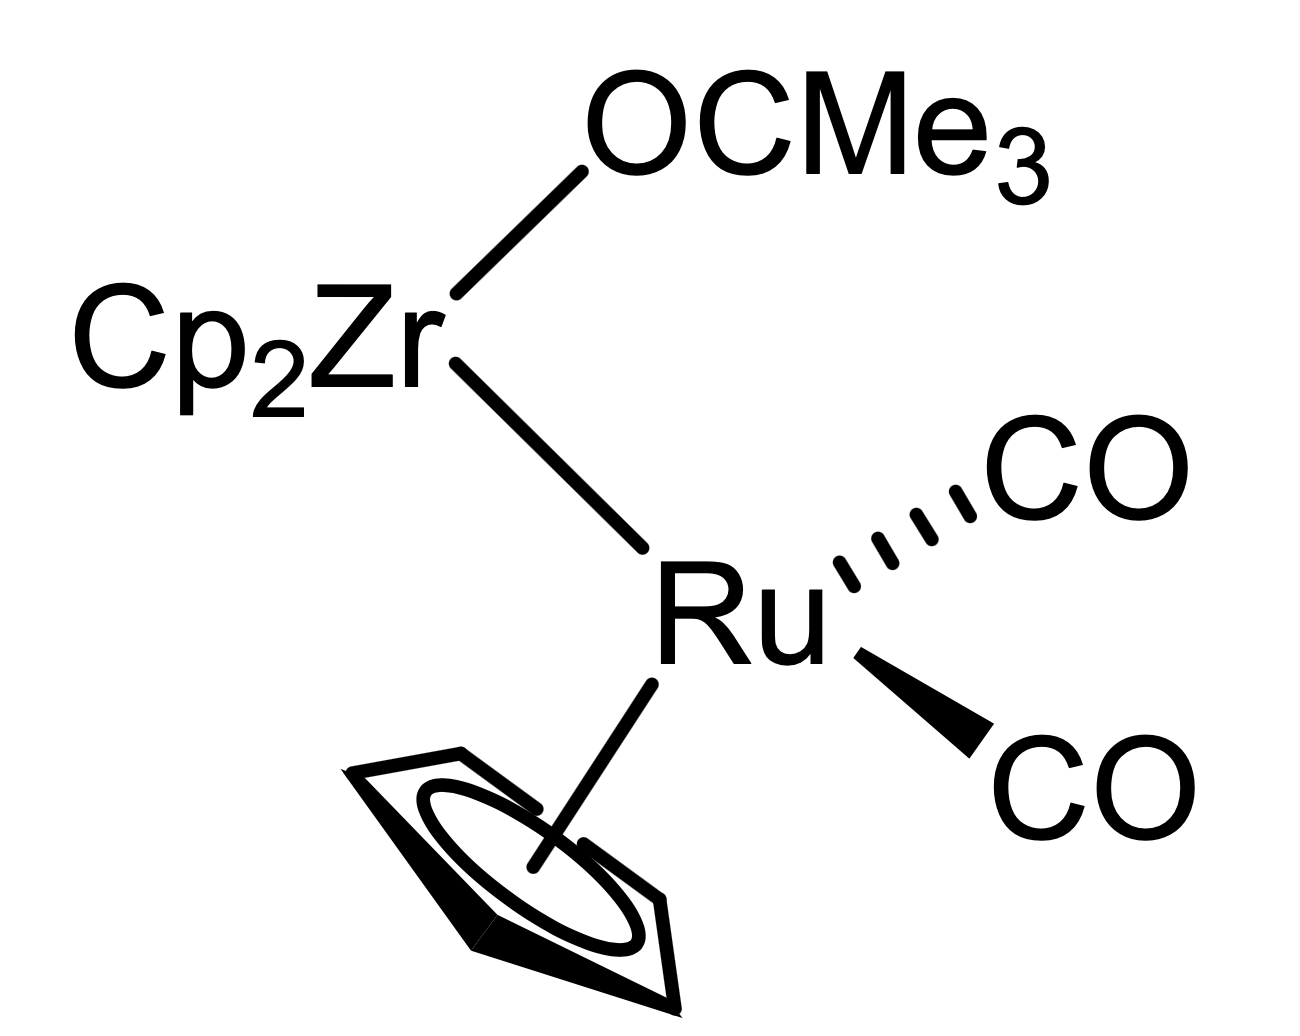
\includegraphics[width=0.24\linewidth]{../ExtFiles/pset1-1-18.png}
        \end{center}
        \begin{proof}[Answer]\leavevmode
            \begin{enumerate}[label={(\roman*)}]
                \item \ce{Zr^3+} (the $t$-butoxide is X-type; both Cp groups are X-type; the \ce{Zr-Ru} bond makes no contribution), and \ce{Ru^+} (both carbonyls are L-type; the Cp is X-type; the \ce{Zr-Ru} bond makes no contribution).
                \item \ce{Zr^3+} is $d^1$, and \ce{Ru^+} is $d^7$.
                \item For the zirconium atom, the $t$-butoxide group is a 1-electron donor, both Cp groups are 5-electron donors, and the \ce{Zr-Ru} bond is a 1-electron donor. Thus, the ligands donate $1\cdot 1+2\cdot 5+1\cdot 1=12$ electrons in total to the zirconium atom. This combined with the above results yields $12+4=16$ as the electron count for the zirconium atom. For the ruthenium atom, both carbonyls are 2-electron donors, the Cp group is a 5-electron donor, and the \ce{Zr-Ru} bond is a 1-electron donor. Thus, the ligands donate $2\cdot 2+1\cdot 5+1\cdot 1=10$ electrons in total. This combined with the above results yields $10+8=18$ as the electron count for the ruthenium atom. It follows that there should be $\frac{36-(16+18)}{2}=1$ extra \ce{Zr-Ru} bond beyond what is shown in the above picture (2 in total).
            \end{enumerate}
        \end{proof}
        \item ${\color{white}hi}$
        \begin{center}
            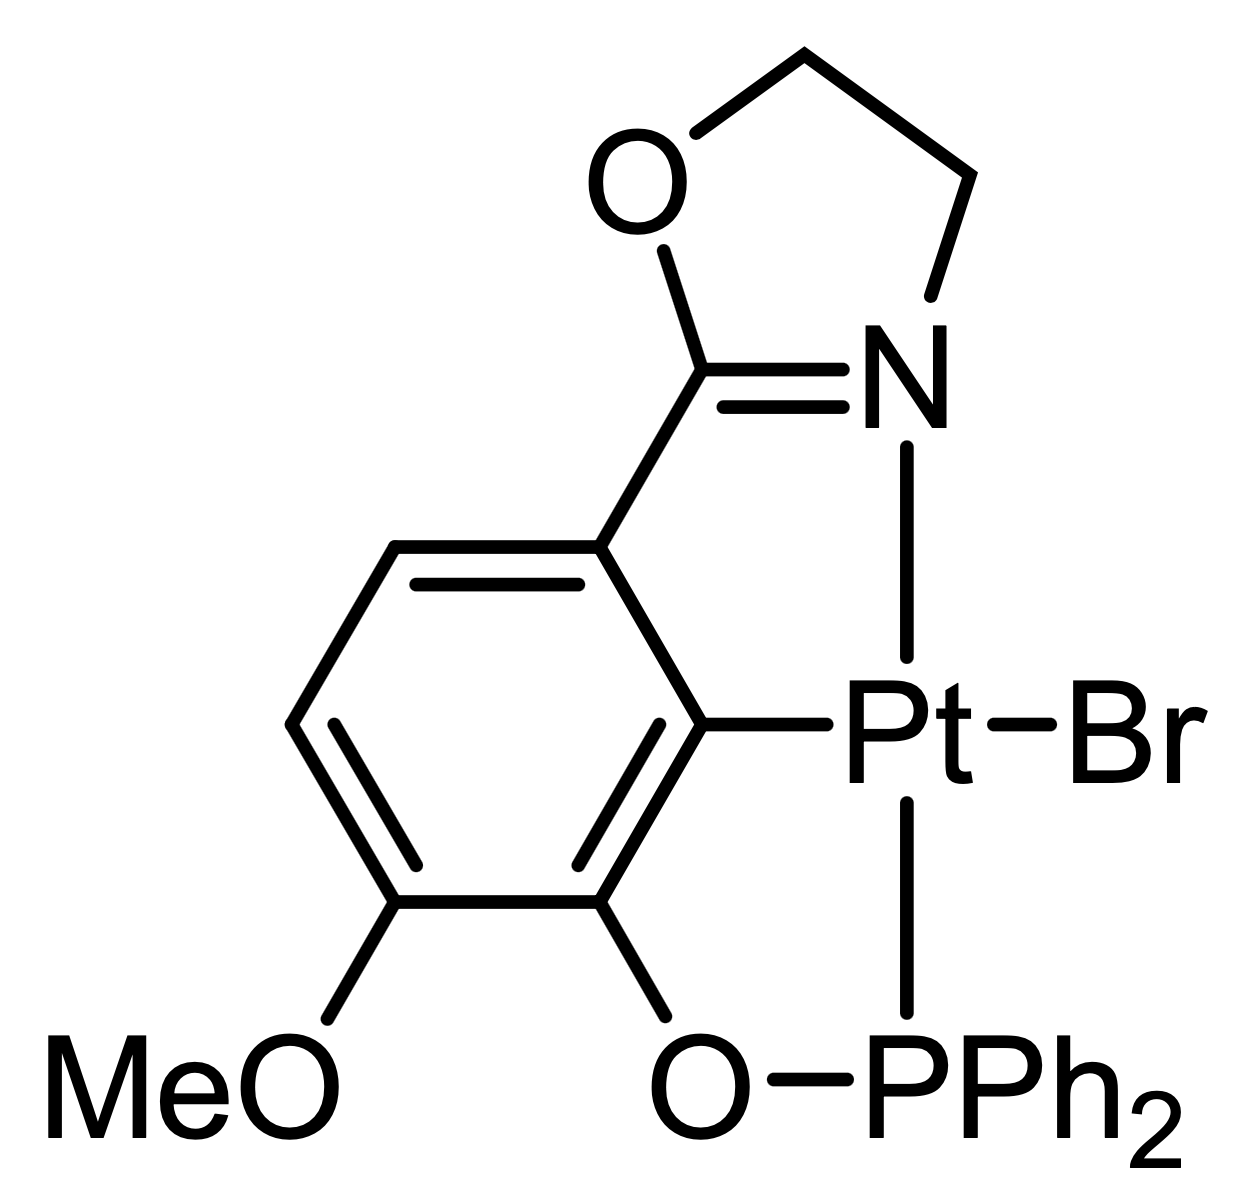
\includegraphics[width=0.25\linewidth]{../ExtFiles/pset1-1-19.png}
        \end{center}
        \begin{proof}[Answer]\leavevmode
            \begin{enumerate}[label={(\roman*)}]
                \item \ce{Pt^2+} (the bromine is X-type; the other ligand is \ce{L2X}-type).
                \item \ce{Pt^2+} is $d^8$.
                \item The bromine is a 1-electron donor, and the other ligand is a 5-electron donor (2 dative bonds plus 1 covalent bond). Thus, the ligands donate $1\cdot 1+1\cdot 5=6$ electrons in total. This combined with the above result yields $6+10=16$ as the electron count.
            \end{enumerate}
        \end{proof}
        \item ${\color{white}hi}$
        \begin{center}
            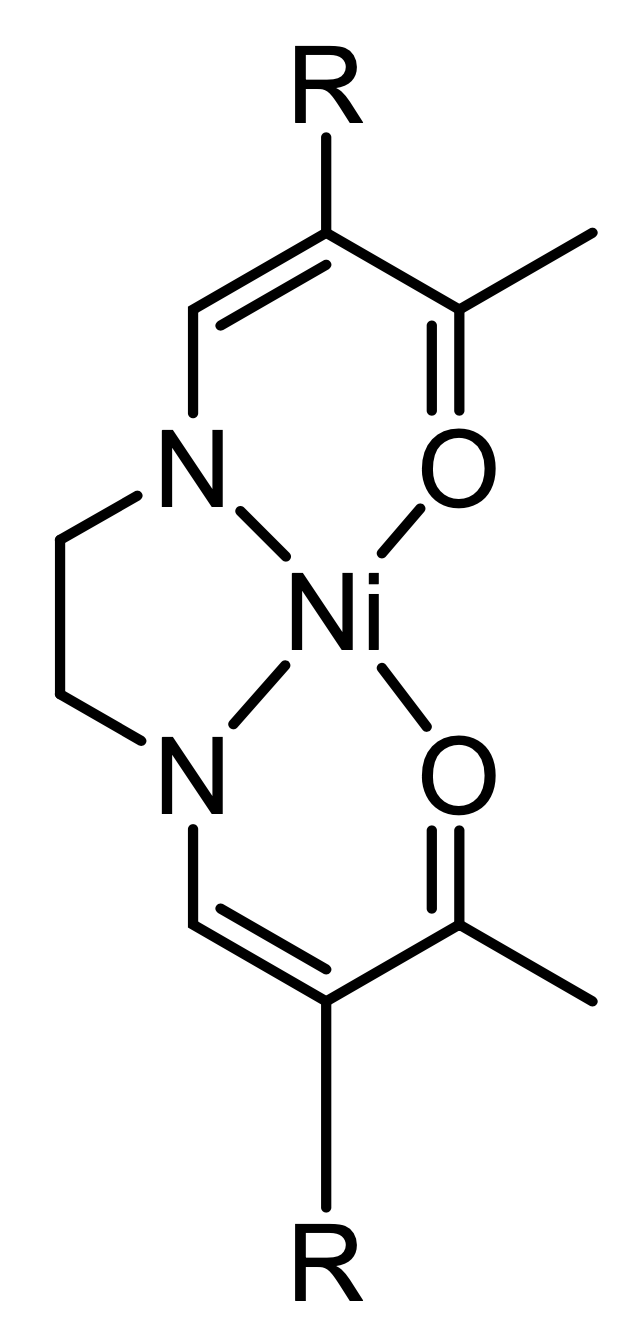
\includegraphics[width=0.16\linewidth]{../ExtFiles/pset1-1-20.png}
        \end{center}
        \begin{proof}[Answer]\leavevmode
            \begin{enumerate}[label={(\roman*)}]
                \item \ce{Ni^2+} (the ligand is \ce{L2X2}-type).
                \item \ce{Ni^2+} is $d^8$.
                \item The ligand is a 6-electron donor (2 dative bonds plus 2 covalent bonds). This combined with the above result yields $6+10=16$ as the electron count.
            \end{enumerate}
        \end{proof}
    \end{enumerate}
    \newpage
    \item For the following pairs of complexes from problem 1, pick and justify based on the trend.
    \begin{enumerate}[label={\alph*)}]
        \item Which complex is more basic and which is more acidic between 2 and 5 (\ce{Co} and \ce{Zr})?
        \begin{proof}[Answer]
            5 is more acidic because it wants to gain two electrons to get to 18 to be more stable, whereas 2 already has 18 electrons, and thus is more basic relatively.
        \end{proof}
        \item Which complex is more likely to be reduced or oxidized between 4 and 15 (both \ce{Fe})?
        \begin{proof}[Answer]
            4 is more likely to be oxidized, and 15 is more likely to be reduced. 4 already has 18 electrons, so it won't want any more. 15 is at 14 electrons, so it would surely stabilize it to gain a few more.
        \end{proof}
        \item Which complex is more likely to have its \ce{M-C} bond hydrolyze between 8 and 12 (\ce{Zr} and \ce{Pd})?
        \begin{proof}[Answer]
            8 is more likely to have its \ce{M-C} bond hydrolyze. In 12, benzene, because it is so stable, is not a great leaving group and the square planar geometry at each metal center is extra stable because of the 16 electron rule (or 18 electrons depending on \ce{Pd-Pd} bonding). However, in 8, the \ce{M-CH3} bond is highly unstable due to the electron count of 14.
        \end{proof}
    \end{enumerate}
    \item Consider the following complex.
    \begin{center}
        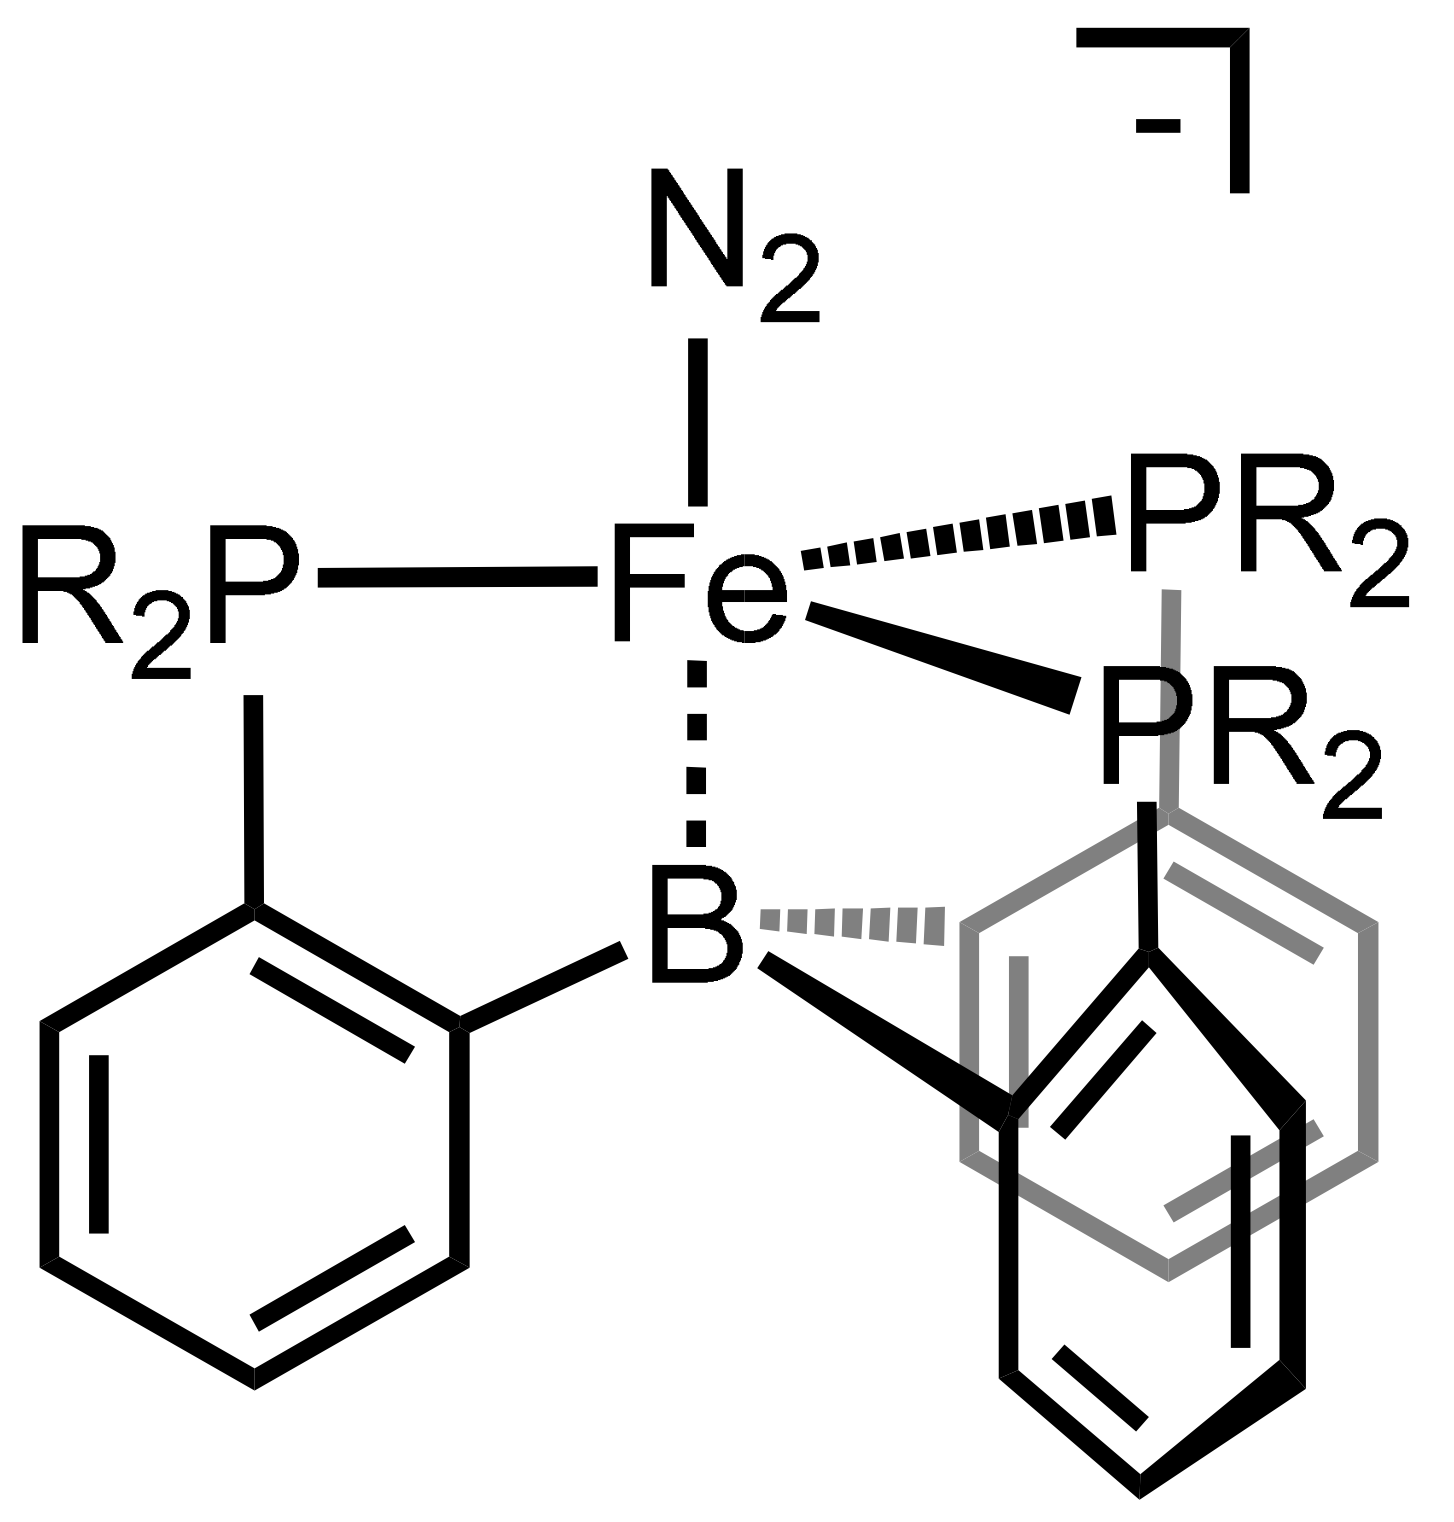
\includegraphics[width=0.23\linewidth]{../ExtFiles/pset1-3.png}
    \end{center}
    \begin{enumerate}[label={\alph*)}]
        \item Assign an oxidation state, $d$ count, overall electron count, and "L/X/Z" formalism.
        \begin{proof}[Answer]
            The oxidation state is \ce{Fe^0} since all ligands form dative bonds.\par
            The $d$ count is $d^8$.\par
            With respect to the overall electron count, \ce{N2} is a 2-electron donor and the bottom ligand is a 6-electron donor. Thus, the electron count is $(2+6)+(8)-(-1)=17$.\par
            The nitrogen is L-type, and the other ligand is \ce{L3Z}-type (assuming that there is a single \ce{Fe-B} bond).
        \end{proof}
        \item Draw 3 different resonance structures for both the \ce{Fe-N2} interaction and the \ce{Fe-B} interactions in this compound (a total of 6) and explain how the oxidation state, $d$ count, and "L/X/Z" formalism changes as a function of resonance structure.
        \begin{proof}[Answer]
            \chemfig[atom sep=1.2em]{Fe-\charge{[extra sep=3pt]45=$\oplus$}{N}~\charge{0=\:}{N}}\quad will be our base Lewis structure of this type. This is an L-type ligand.\\[9pt]
            \chemfig[atom sep=1.2em]{Fe=\charge{[extra sep=3pt]45=$\oplus$}{N}=\charge{[extra sep=3pt]90=\:,-90=\:,45=$\ominus$}{N}}\quad exhibits no changes in oxidation state, $d$ count, or type\footnote{\label{fnt:2electronMultipleBond}As per Sophie's explanation in office hours, there are not actually more electrons in the \ce{M-C} double bond in this resonance structure; rather, it simply shows up spectroscopically as shorter, so we denote this still 2-electron bond as having bond order 2. We have a similar case for the other resonance structures.}.\\[9pt]
            \chemfig[atom sep=1.2em]{Fe~\charge{[extra sep=3pt]45=$\oplus$}{N}-\charge{[extra sep=3pt]90=\:,45[xshift=1mm]=2$\ominus$,0=\:,-90=\:}{N}}\qquad exhibits no changes in oxidation state, $d$ count, or type.\\[15pt]
            \chemfig[atom sep=1.2em]{Fe-[,,,,white]B}\quad will be our base Lewis structure of this type. This is not any type of ligand as no bond is present.\\[9pt]
            \chemfig[atom sep=1.2em]{Fe-\charge{45=$\ominus$}{B}}\quad exhibits no changes in oxidation state or $d$ count. This is a Z-type ligand.\\[9pt]
            \chemfig[atom sep=1.2em]{Fe=\charge{45[xshift=1mm]=2$\ominus$}{B}}\qquad exhibits no changes in oxidation state, $d$ count, or type (still Z-type).
        \end{proof}
        \item How might the valence of the species differ from the oxidation state in the resonance structure depicted in the chem draw above?
        \begin{proof}[Answer]
            % Assuming the \ce{Fe-B} interaction to be a single bond, the valence would be $2+$ whereas the oxidation state is still 0. This is because two of the iron's electrons are engaged in bonding with the boron, but would retreat to the metal center should the bonds be homolytically cleaved.

            For the reason discussed in Footnote \ref{fnt:2electronMultipleBond}, the valence would not change in any of the \ce{Fe-N} resonance structures. However, depending on the nature and extent of the \ce{Fe-B} bonding, it could well increase when bonding first occurs (although, again, it will not likely change within the bonded resonance structures).
        \end{proof}
    \end{enumerate}
    \item For the following ligands, draw all possible resonance structures with formal charges, indicate the number of electrons donated to a generic metal complex, and assign the ligand to its appropriate "L/X/Z" formulation.
    \begin{enumerate}[label={\alph*)}]
        \item \ce{PR3}.
        \begin{proof}[Answer]
            Structure:
            \begin{center}
                \chemfig{M-P(-[2,0.7]R)(-[,0.7]R)(-[6,0.7]R)}
            \end{center}
            2-electron donor.\par
            L-type ligand.
        \end{proof}
        \item \ce{CO}.
        \begin{proof}[Answer]
            Resonance structures:
            \vspace{0.5em}
            \begin{center}
                \schemestart
                    \chemfig{M-C~\charge{0=\:,45[xshift=1mm,yshift=1mm]=$\oplus$}{O}}
                    \arrow{<->}
                    \chemfig{M=C=\charge{45=\:,-45=\:}{O}}
                    \arrow{<->}
                    \chemfig{M~C-\charge{0=\:,90=\:,-90=\:,45[xshift=1mm,yshift=1mm]=$\ominus$}{O}}
                \schemestop
            \end{center}
            2-electron donor.\par
            L-type ligand.
        \end{proof}
        \item \ce{NO}.
        \begin{proof}[Answer]
            Resonance structures:
            \vspace{0.5em}
            \begin{center}
                \schemestart
                    \chemleft{[}
                        \chemfig{M-\charge{45[xshift=1mm,yshift=1mm]=$\oplus$}{N}~\charge{0=\:,45[xshift=1mm,yshift=1mm]=$\oplus$}{O}}
                    \chemright{]^+}
                    \arrow{<->}
                    \chemleft{[}
                        \chemfig{M=\charge{45[xshift=1mm,yshift=1mm]=$\oplus$}{N}=\charge{45=\:,-45=\:}{O}}
                    \chemright{]^+}
                    \arrow{<->}
                    \chemleft{[}
                        \chemfig{M~\charge{45[xshift=1mm,yshift=1mm]=$\oplus$}{N}-\charge{0=\:,90=\:,-90=\:,45[xshift=1mm,yshift=1mm]=$\ominus$}{O}}
                    \chemright{]^+}
                \schemestop\\[1em]
                \chemfig{M-[:30]\charge{90=\:}{N}=[:-30]\charge{0=\:,-90=\:}{O}}
            \end{center}
            The top set of resonance structures are 3-electron-donating L-type ligands. The bottom structure is a 1-electron-donating X-type ligand.
        \end{proof}
        \item \ce{C3H5}.
        \begin{proof}[Answer]
            Resonance structures:
            \begin{center}
                \schemestart
                    \chemfig{M-[:105,2]\phantom{i}-[:-150,0.5,,,white]C(-[:150]H)(-[6]H)=[:30]C(-[2]H)-[:-30]C(-[:30]H)(-[6]H)}
                    \arrow{<->}
                    \chemfig{M-[:75,2]\phantom{i}-[:150,0.5,,,white]\phantom{C}-[:-150,,,,white]C(-[:150]H)(-[6]H)-[:30]C(-[2]H)=[:-30]C(-[:30]H)(-[6]H)}
                \schemestop
            \end{center}
            3-electron donor.\par
            LX-type ligand.
        \end{proof}
        \newpage
        \item "\ce{NR}."
        \begin{proof}[Answer]
            Resonance structures:
            \vspace{0.5em}
            \begin{center}
                \schemestart
                    \chemfig{M-[:30]\charge{45=\:,135=\:,90[yshift=1mm]=$\ominus$}{N}-[:-30]R}
                    \arrow{<->}
                    \chemfig{M=[:30]\charge{90=\:}{N}-[:-30]R}
                    \arrow{<->}
                    \chemfig{M~\charge{45[xshift=1mm,yshift=1mm]=$\oplus$}{N}-R}
                \schemestop
            \end{center}
            2-electron donor.\par
            \ce{X2}-type ligand.
        \end{proof}
    \end{enumerate}
    \item Predict the spin state, $\mu_\text{eff}$, and $\chi T$ values for the following ions in the indicated geometry.
    \begin{enumerate}[label={\alph*)}]
        \item Tetrahedral \ce{Mn}(II).
        \begin{proof}[Answer]
            High spin $d^5$ (tetrahedral has small orbital splitting). Thus,
            \begin{align*}
                \mu_\text{eff} &= 2\sqrt{\frac{5}{2}\left( \frac{5}{2}+1 \right)}&
                    \chi T &= \frac{2^2}{8}\left( \frac{5}{2}\left( \frac{5}{2}+1 \right) \right)\\
                &= \sqrt{35}&
                    &= \frac{35}{8}
            \end{align*}
        \end{proof}
        \item Octahedral \ce{Ir}(III).
        \begin{proof}[Answer]
            Low spin $d^6$ (high oxidation state implies large $\Delta$, so low spin). Thus,
            \begin{align*}
                \mu_\text{eff} &= 2\sqrt{0(0+1)}&
                    \chi T &= \frac{2^2}{8}(0(0+1))\\
                &= 0&
                    &= 0
            \end{align*}
        \end{proof}
        \item Octahedral \ce{Ru}(III).
        \begin{proof}[Answer]
            Low spin $d^5$ (high oxidation state implies large $\Delta$, so low spin). Thus,
            \begin{align*}
                \mu_\text{eff} &= 2\sqrt{\frac{1}{2}\left( \frac{1}{2}+1 \right)}&
                    \chi T &= \frac{2^2}{8}\left( \frac{1}{2}\left( \frac{1}{2}+1 \right) \right)\\
                &= \sqrt{3}&
                    &= \frac{3}{8}
            \end{align*}
        \end{proof}
        \item Square planar \ce{Co}(II).
        \begin{proof}[Answer]
            Low spin $d^7$ (square planar has large orbital splitting). Thus,
            \begin{align*}
                \mu_\text{eff} &= 2\sqrt{\frac{1}{2}\left( \frac{1}{2}+1 \right)}&
                    \chi T &= \frac{2^2}{8}\left( \frac{1}{2}\left( \frac{1}{2}+1 \right) \right)\\
                &= \sqrt{3}&
                    &= \frac{3}{8}
            \end{align*}
        \end{proof}
        \newpage
        \item Square planar \ce{Pt}(II).
        \begin{proof}[Answer]
            Low spin $d^8$ (square planar has large orbital splitting). Thus,
            \begin{align*}
                \mu_\text{eff} &= 2\sqrt{0(0+1)}&
                    \chi T &= \frac{2^2}{8}(0(0+1))\\
                &= 0&
                    &= 0
            \end{align*}
        \end{proof}
        \item Octahedral \ce{Ni}(II).
        \begin{proof}[Answer]
            High spin $d^8$ (low oxidation state implies small $\Delta$, so high spin). Thus,
            \begin{align*}
                \mu_\text{eff} &= 2\sqrt{1(1+1)}&
                    \chi T &= \frac{2^2}{8}(1(1+1))\\
                &= 2\sqrt{2}&
                    &= 1
            \end{align*}
        \end{proof}
        \item Tetrahedral \ce{Cr}(II).
        \begin{proof}[Answer]
            High spin $d^4$ (tetrahedral has small orbital splitting). Thus,
            \begin{align*}
                \mu_\text{eff} &= 2\sqrt{2(2+1)}&
                    \chi T &= \frac{2^2}{8}(2(2+1))\\
                &= 2\sqrt{6}&
                    &= 3
            \end{align*}
        \end{proof}
    \end{enumerate}
    \item Predict the relative radii between the two ions listed (i.e., same, larger, or smaller) assuming an octahedral field, and rationalize your choice.
    \begin{enumerate}[label={\alph*)}]
        \item Low spin \ce{Fe}(II) or high spin \ce{Fe}(II).
        \begin{proof}[Answer]
            High spin \ce{Fe}(II) has a larger radius than low spin \ce{Fe}(II) because the $e_g$ orbitals are antibonding, so having more antibonding electrons both pushes the bounds of the atom (increasing the atomic radius) and weakens bonds (increasing the covalent radius).
        \end{proof}
        \item \ce{Mn}(II) or \ce{Mn}(III).
        \begin{proof}[Answer]
            \ce{Mn}(II) has a larger radius than \ce{Mn}(III) because having more electrons means more intra-orbital repulsions, all of which push the bounds of the atom.
        \end{proof}
        \item Low spin \ce{Ti}(II) or high spin \ce{Ti}(II).
        \begin{proof}[Answer]
            The radius is the same (low spin equals high spin for $d^2$ complexes).
        \end{proof}
        \item \ce{Zr}(IV) or \ce{Zr}(III).
        \begin{proof}[Answer]
            \ce{Zr}(III) has a larger radius than \ce{Zr}(IV) for the same reasons listed in part (b).
        \end{proof}
    \end{enumerate}
    \item The isolobal analogy is frequently used to help relate seemingly disparate fragments. Utilize this analogy to compare the bonding in terminal nitride (\ce{N}) and alkylidyne (\ce{CR}) complexes.
    \begin{proof}[Answer]
        Since we have \chemfig[atom sep=1.2em]{M=\charge{45=\:,-45=\:}{N}}\quad and \chemfig[atom sep=1.2em]{M=\charge{90=\:}{C}-R} for how the two ligands bond, we can assume based on the fact that the two ligands are isoelectronic and isolobal (simply replace a lone pair in the nitride with the bond in the alkylidyne, or vice versa) that they have similar bonding, stability, and chemical properties.
    \end{proof}
    \item Read \textcite{bib:CBC}. Based on this paper, answer the following questions.
    \begin{enumerate}[label={\alph*)}]
        \item In your own words, explain the reasons why the author considers a different form of bond classification necessary.
        \begin{proof}[Answer]
            % Oxidation state is difficult (homopolar ponds are neglected, there is debate about the inclusion of other bonds). Coordination number is difficult (can treat differently very similar compounds, such as \ce{Mo(CO)6}, \ce{Mo($\eta${-}C6H6)(CO)3}, and \ce{Mo($\eta${-}C6H6)2}). In short, the classification of inorganic compounds was made under the assumption that all compounds could be described as ionic, like the relatively simple ionic ones first studied.

            The ionic method relies heavily on the calculation of the metal center's oxidation state and coordination number. However, while these two quantities suitably treated the known inorganic compounds of the early twentieth century (i.e., ones that were easily described as ionic), they play less nicely with the oft covalently bonded complexes of today. As such, \textcite{bib:CBC} created the covalent bond classification method to solve issues arising from these two quantities.\par
            In brief, the problems with the oxidation state stem from the fact that calculations of it are debatable for some bonds, and they flat-out neglect homopolar bonds. The problems with coordination number mainly surround the fact that it can treat very similar compounds quite differently (for example, \ce{Mo(CO)6}, \ce{Mo($\eta${-}C6H6)(CO)3}, and \ce{Mo($\eta${-}C6H6)2} have coordination numbers of 6, 9, and 12, respectively).
        \end{proof}
        \item Is it more common to have a \ce{MoL2X4} compound or \ce{MoL4X2} compound?
        \begin{proof}[Answer]
            It is more common to have a \ce{MoL2X4} compound than a \ce{MoL4X2} compound, as can be read from Figure 1 on \textcite[128]{bib:CBC}.
        \end{proof}
        \item What are the differences in the ligand bonding orbitals for L-, X-, and Z-type ligands?
        \begin{proof}[Answer]
            % X-type: Singly occupied orbital on the ligand which requires one electron from the metal center to form a two-electron covalent bond. Can have multiple such orbitals on a single ligand; for example, carbenes (\ce{=CR2}) have two.
            % L-type: Ligand based orbital with two electrons; both are donated to an empty orbital on the metal center. Can have multiple such orbitals on a single ligand; for example, ethylenediamine has two.
            % Z-type: Empty ligand orbital that accepts electron pair donation from the metal.

            L-type: Two electrons are donated from a ligand-based orbital to an empty orbital on the metal center via the formation of a single dative bond.\par
            X-type: One electron is donated from a singly occupied ligand-based orbital to the metal center via the formation of a single covalent bond that also requires one electron from the metal center.\par
            Z-type: An empty ligand orbital accepts an electron pair from the metal via the formation of a single bond.
        \end{proof}
        \item Draw \ce{L2}, \ce{LX}, and \ce{X2} forms of a sulfate ion bound to a generic metal \ce{M}.
        \begin{proof}[Answer]
            ${\color{white}hi}$
            \begin{figure}[H]
                \centering
                \begin{subfigure}[b]{0.3\linewidth}
                    \centering
                    \chemfig{M?-[1,,,,stealth-]\charge{45=\:,-135=\:}{O}=[7]S(-[1]\charge{45=\:,135=\:,-45=\:,90[yshift=1mm]=$\ominus$}{O})(-[7]\charge{45=\:,-45=\:,-135=\:,-90[yshift=-1mm]=$\ominus$}{O})=[5]\charge{-45=\:,135=\:}{O}?[,,{stealth-}]}
                    \vspace{0.5em}
                    \caption{\ce{L2} form.}
                    \label{fig:pset1-8d-answera}
                \end{subfigure}
                \begin{subfigure}[b]{0.3\linewidth}
                    \centering
                    \chemfig{M?-[1]\charge{45=\:,135=\:}{O}-[7]S(=[1]\charge{0=\:,90=\:}{O})(-[7]\charge{45=\:,-45=\:,-135=\:,-90[yshift=-1mm]=$\ominus$}{O})=[5]\charge{-45=\:,135=\:}{O}?[,,{stealth-}]}
                    \vspace{0.5em}
                    \caption{\ce{LX} form.}
                    \label{fig:pset1-8d-answerb}
                \end{subfigure}
                \begin{subfigure}[b]{0.3\linewidth}
                    \centering
                    \chemfig{M?-[1]\charge{45=\:,135=\:}{O}-[7]S(=[1]\charge{0=\:,90=\:}{O})(=[7]\charge{0=\:,-90=\:}{O})-[5]\charge{-45=\:,-135=\:}{O}?}
                    \vspace{0.5em}
                    \caption{\ce{X2} form.}
                    \label{fig:pset1-8d-answerc}
                \end{subfigure}
                \caption{Different ways sulfate can bind to a metal center.}
                \label{fig:pset1-8d-answer}
            \end{figure}
        \end{proof}
        \item What does valency/valence number mean and how does that differ from oxidation state? What type of complex has a different valence number and oxidation state? Similarly, what does ligand bond number mean and how does this differ from coordination number? Give an example of a ligand where coordination number and ligand bond number differ.
        \begin{proof}[Answer]
            \textbf{Valency}: The number of X-functions on the ligands, where an X-function is a singly occupied orbital on the ligand which requires one electron from the metal center to form a two-electron covalent bond. \emph{Also known as} \textbf{valence number}, \textbf{V.N.}\par
            \textbf{Oxidation state}: The number of electrons that the metal center gains or loses when all bonds are homolytically and ionically cleaved. \emph{Also known as} \textbf{O.S.}\par
            Unlike the O.S., the V.N. includes homopolar (e.g., \ce{M-M}) bonds and cannot, by definition, be negative.\par
            \textbf{Ligand bond number}: The sum of the number of X-functions and the number of L-functions on the ligands, where an X-function is defined as above and an L-function is a single ligand orbital occupied by two electrons, both of which are donated to an empty orbital on the metal center during bonding. \emph{Also known as} \textbf{L.B.N.}\par
            \textbf{Coordination number}: The number of other atoms bonded to the metal center. \emph{Also known as} \textbf{C.N.}\par
            The L.B.N. and C.N. differ when the metal ligand bonding is more complex. For example, one place where the two differ is in any coordination complex with a double bonded ligand (that's two X-functions but only one ligand).
        \end{proof}
        \item What does two ligands being in the same ligand domain mean? How does this relate to the isolobal analogy from question 7?
        \begin{proof}[Answer]
            It means that they have similar steric and electronic properties. Although ligands in the same domain may not be isolobal (or isoelectronic) and have \emph{that} kind of close similarity, they do share more than a passing resemblance.
        \end{proof}
    \end{enumerate}
\end{enumerate}




\end{document}